\documentclass[12pt]{examnotes}

\header{{ECS3704 Public Economics}}
%%%%%%%%%%%%%%%%%%%%%%%%%%%%%%%%%%%%%%%

\begin{document}

\obeylines

\setlength\baselineskip{15pt}

\h{Study Unit 1}

\sh{6 Assumptions of benchmark model }
\ra Two individuals, both are suppliers of fixed quantities of capital and labour, producers of 2 commodities and consumers of 2 commodities.
\ra Fixed tastes and no external effects on consumption. (Indifference curves are continuous, convex, non-intersecting, diminishing MRS)
\ra Unlimited factor substitutions. (Isoquants are diminishing MRTS, constant returns to scale)
\ra Consumers maximise utility, and producers maximisers profit, both have prefect knowledge, and are fully mobile. 
\ra Competitive commodity and factor markets. (price takers)
\ra Assumptions together ensure existence, uniqueness sand stability of a general equilibrium.

\sh{The benchmark model and allocative efficiency}
\ra Allocative efficiency: limited resource of country are allocated in accordance with the wishes of its consumers. 
\ra An interaction between consumption activities of individuals and the production activities of producers.
{\bf 3 Conditions:}
\ra {\bf Condition 1 - Equilibrium in production}
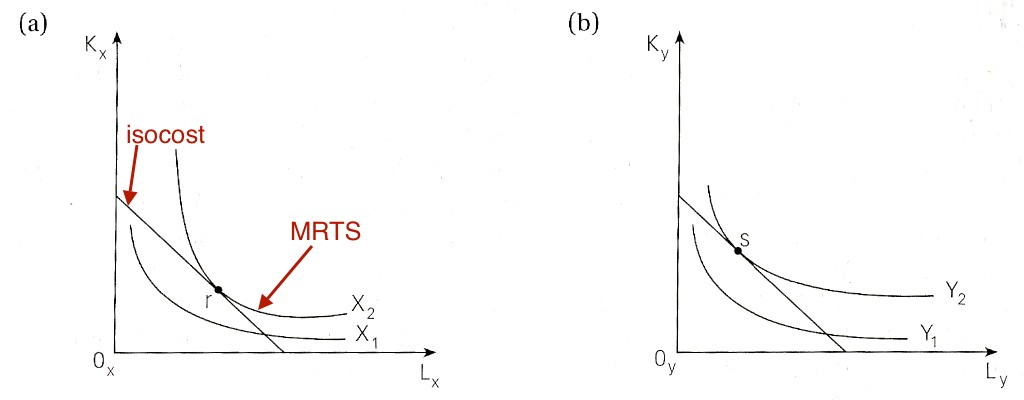
\includegraphics[scale=0.4]{./imgs/21.jpg}
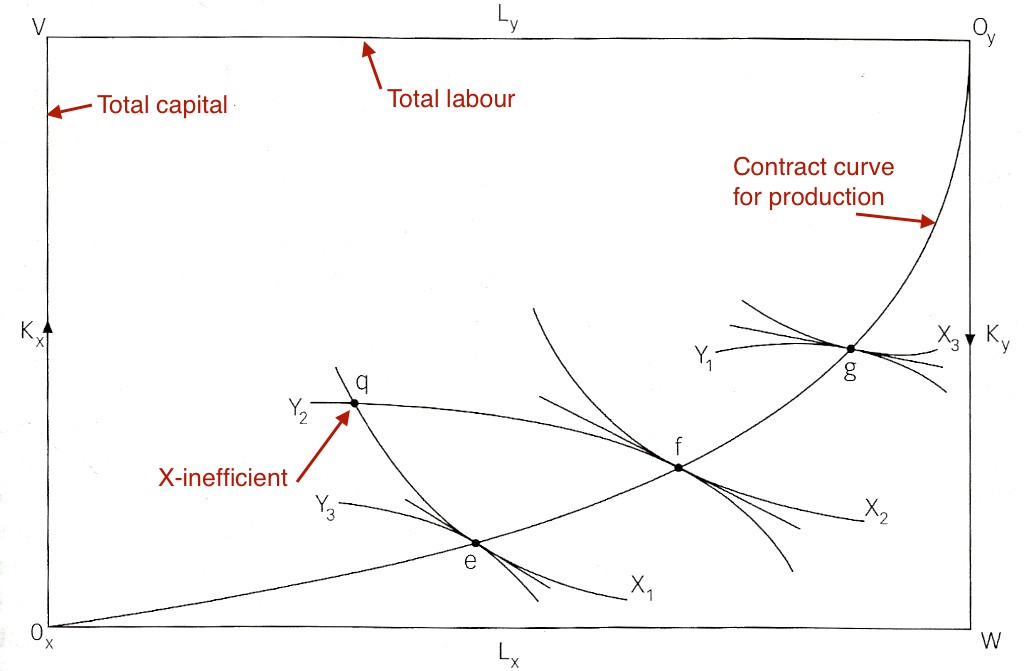
\includegraphics[scale=0.3]{./imgs/22.jpg}
\ra Production activities must be Pareto optimal. Not possible to increase output any one commodity without decreasing the output of at least one other commodity. 
\ra Under perfect competition $P_X=MC_x$  
\vspace{3pt}
\ra $MRTS^x_{lk}=\displaystyle\frac{MPL_x}{MPK_x}=\frac{w}{r}$
\vspace{3pt}
\ra Under prefect competition $MRTS_{lk}^x=\frac{w}{r}=MRTS_{lk}^y$
\ra Each point on contract curve is Pareto optimal.
\ra MRPT = Marginal rate of product transformation.
\vspace{3pt}
\ra $MRPT_{xy}=\displaystyle\frac{MC_x}{MC_y}=\frac{P_x}{P_y}=\frac{\Delta Y}{\Delta X}$. Slope of tangent to PPC.
\ra 
\vspace{3pt}
\ra $MC_x=\displaystyle\frac{\Delta TC_x}{\Delta X}$
\vspace{3pt}

\vspace{6pt}
\ra {\bf Condition 2 - Equilibrium in consumption}
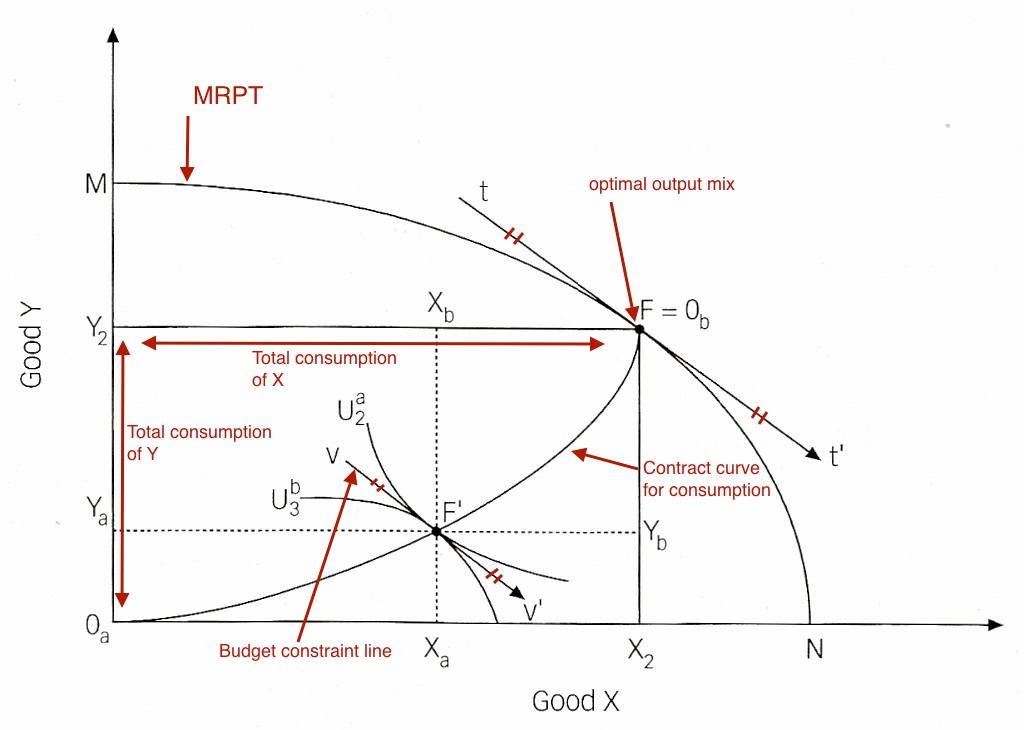
\includegraphics[scale=0.4]{./imgs/24.jpg}
\ra Economic efficiency in consumption implies no interpersonal re-allocation of commodities can increase the utility of a consumers without thereby decreasing the utility of another. 
\ra Each consumer maximise utility subject to budget constraint.
\ra $MRS^a_{xy}=\displaystyle \frac{P_x}{P_y}=MRS^b_{xy}$.
\ra Contract curve for consumption. Indifference curve of consumers are tangent. 
\ra How much each individual consumes depends on:
\rn{1} Their relative preference or tastes for the commodities
\rn{2} There income which depends on the the initial resources (K and L) they own.

\ra {\bf Condition 3 - Simultaneous equilibrium for producers and consumers}
\ra Top-level condition.
\ra Producers and consumers achieve equilibrium simultaneously.
\ra $MRPT_{xy}=\displaystyle\frac{MC_x}{MC_y}=\frac{P_x}{P_y}=MRS^a_{XY}=MRS^b_{xy}=MRS^a_{xy}$.
\ra Point $F$ is Pareto-optimal top-level equilibrium.

\sh{Efficiency and economic growth}
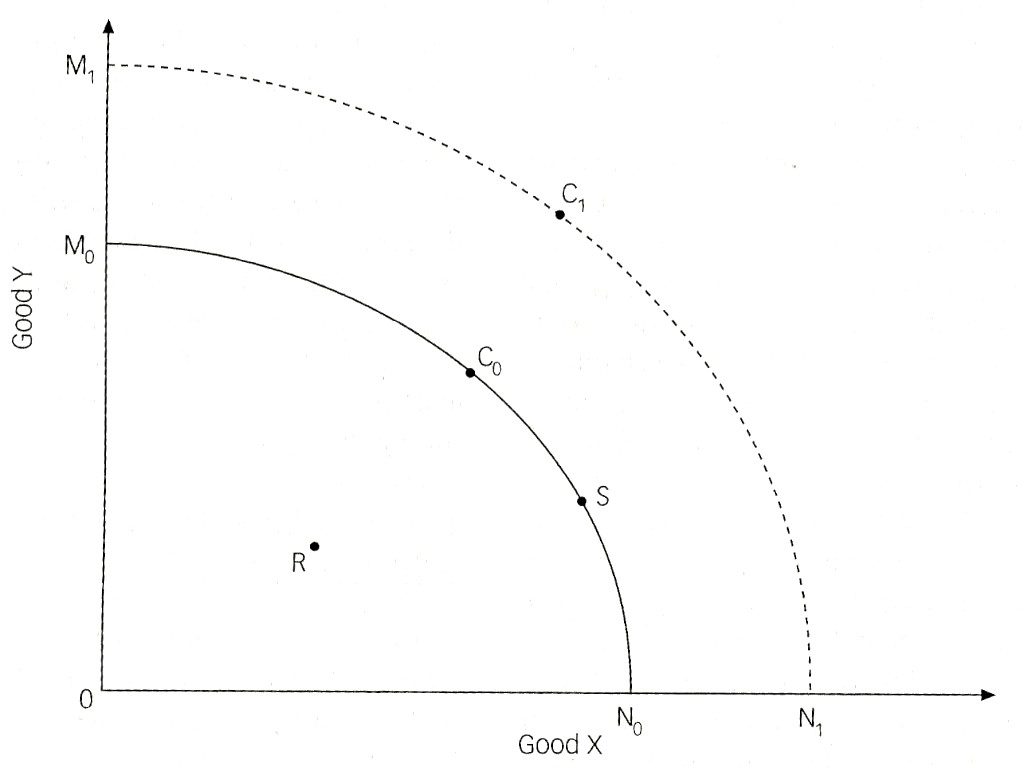
\includegraphics[scale=0.25]{./imgs/25.jpg}
\ra X-efficiency = technical efficiency, existing resources are utilised in the most efficient manner and is on the PPC.
\ra Results from lack of motivation by producing agents, lack of market information, incomplete knowledge of production functions, incomplete specification of labour contracts.
\ra X-efficiency ensures that society is on the PPC.
\ra An outward shift of PPC from increases in savings, investment, human capital formation, technological  inventions, increase in labour of different skills.
\ra Non-maximising behaviour can be found under monopoly.

\sh{Market failure}
\ra Lack of information 
\ra Frictions and lags in adjustments
\ra Incomplete markets
\ra Non-competitive markets
\ra Macroeconomic instability
\ra Distribution of income

\sh{Allocative function}
\ra Stems from market failures distorting the allocation of resource in an economy, particularly incomplete and non-efficient markets.
\ra  Incomplete markets. Public and mixed goods. Positive and negative externalities.
\ra Non-efficient markets. Artificial and natural monopolies.

\sh{Distributive function}
\ra Correct fairness of Pareto optimal outcomes.
\ra Considerable disagreement about this function.
\ra Governments use a combination of tax, transfer payments and subsidies to alter market outcomes.

\sh{Stabilisation function}
\ra Macroeconomic objectives, rate of economic growth, full employment,prices stability, management of balance-of-payments.
\ra Keynesian stabilisation:
\rn{1} Market economy is inherently unstable
\rn{2} Macroeconomic instability is a highly costly market failure
\rn{3} Governments are able to stabilise the economy by means of appropriate macroeconomic policies.

\sh{Direct government intervention}
\ra Actual participation of movement in the economy, taxing individuals and companies, borrow in financial markets.

\sh{Indirect government intervention}
\ra Regulatory function. Laws that gives rise to market outcomes that are different from those in the absence of intervention.
\ra Regulatory interventions do not show up in the national or government accounts, but whose total affect us as important as direct intervention.

\sh{Government failure}
\ra \note{incomplete}

\h{Study Unit 2}

\sh{Characteristics of private goods}
\ra Rivalry in consumption: one individuals consumption reduces availability to other individuals.
\ra Excludability: consumption of a private good can be restricted to given individuals by assignment of property rights typically by payment.
\ra These force customers to revel their preferences and create allocative efficiency.

\sh{Explain the equilibrium of a private good with the aid of a diagram.}
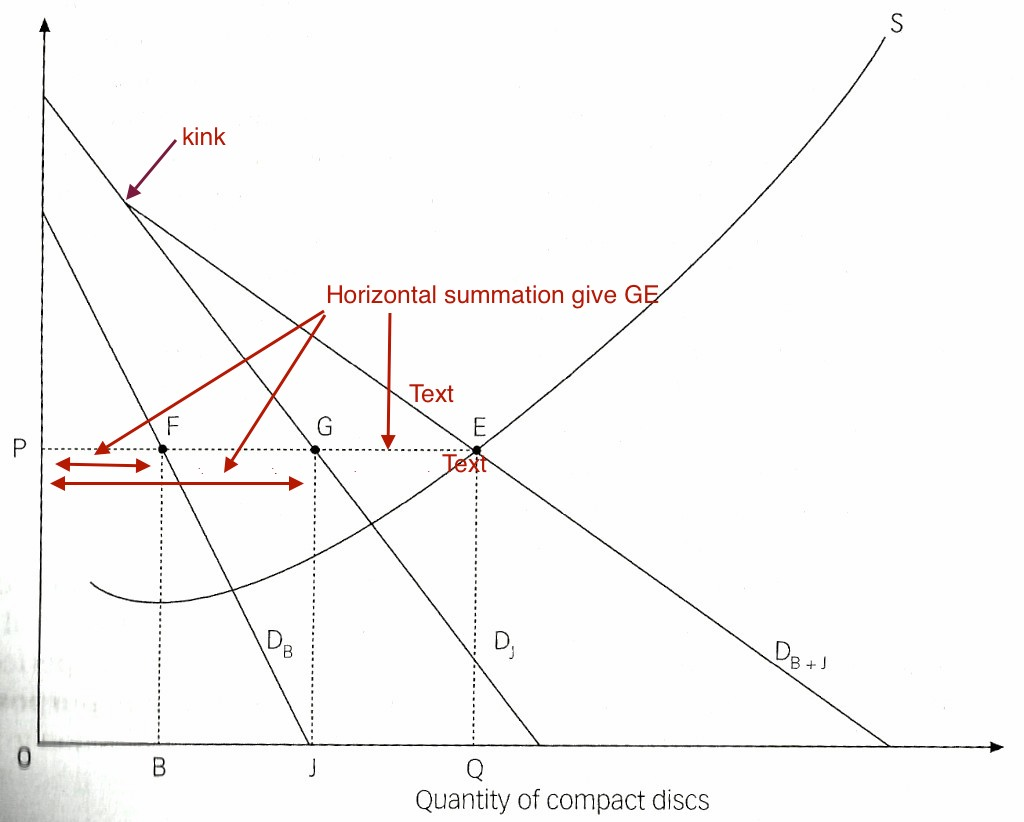
\includegraphics[scale=0.25]{./imgs/31.jpg}
\ra Efficient production under competitive conditions requires consumers reveal their preferences for goods and services and are forced to dues so because of a private good's rivalry and excludability.
\ra $D_B$ + $D_J$ gives $D_{B+J}$ (sum of individual quantities demanded horizontally at each price.)
\ra Equilibrium at E at Price P
\ra Equilibrium quantity 0Q 
\ra In equilibrium $MU_b=MU_j = MC = P$ which is optimal provision.
\ra Consumers are price-takers and quantity-adjusters
{\bf Conditions for the optimal allocation of private goods.}
\ra Condition of efficient supply (optimal provision). MU = MC for each consumer.
\ra Efficient pricing rule to maximise profit. P = MC. 

\sh{Pure public (social) goods}
\de{Non-rivalry}
\ra Street lighting.
\rn{1} Indivisible, one persons consumption does not reduce the quantity available (MC=0). 
\rn{2} Excluding anyone from consuming a non-rival good is Pareto-inefficient.

\de{Non-excludability}
\ra  It is impossible to exclude particular individuals from consuming goods or not possible to assign property rights.
\ra Street lights, national defence as examples
\ra Criteria are stringent and grey arrears abound, technology also changes classification over time. 
\ra Non-excludability is advocated commonly because its costly enforce excludability.
 
\sh{Explain how the equilibrium of a pure public good is derived.}
\vspace{6pt}
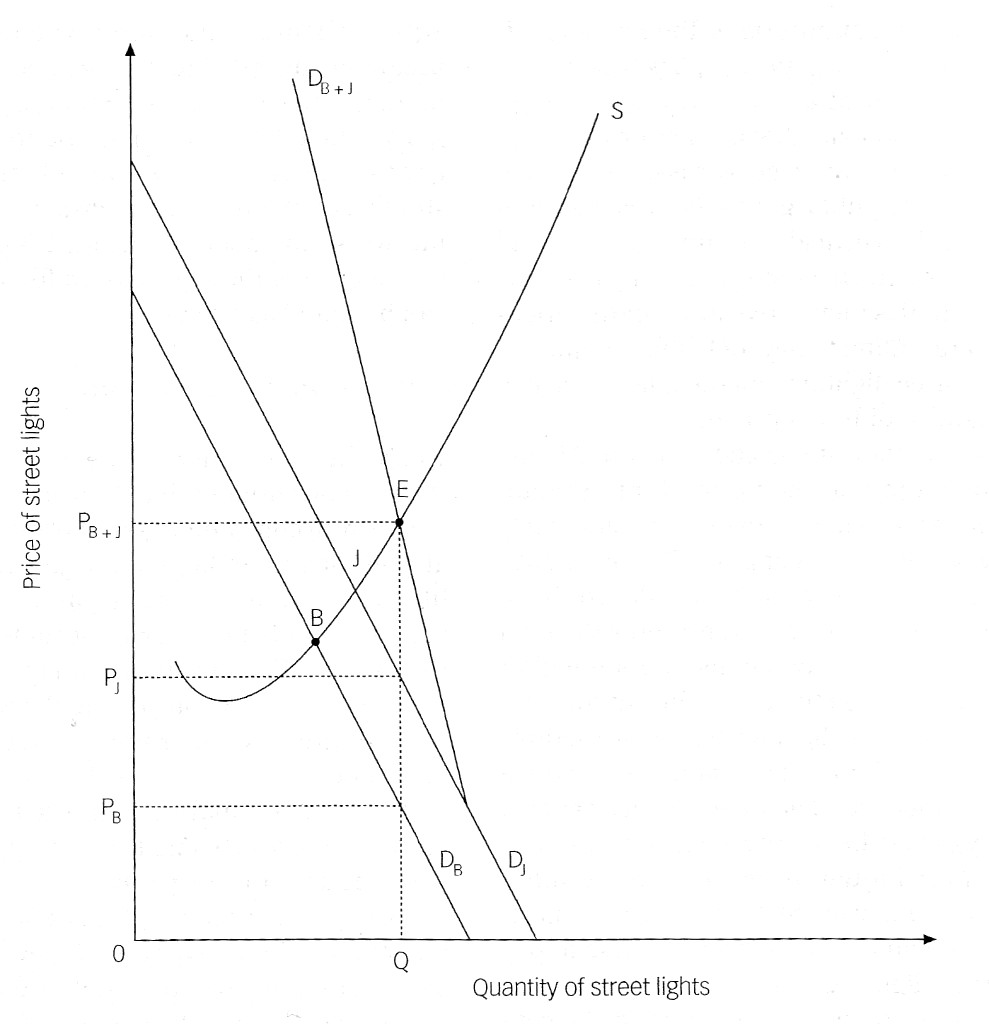
\includegraphics[scale=0.3]{./imgs/32.jpg}
\ra Pseudo demand curves, because consumers can't reveal their preferences accurately.
\ra Vertical summing of individual demand curves, due to indivisibility and non-excludability 
\ra Consumers are quantity-takers and price-adjusters
\ra Equilibrium at E and quantity QE available to both
\ra Individuals willing to pay price (tax) $0P_B$ and  $0P_A$ equal to their individual MU's.
\ra $P^x_{B+J}=MC^x=MU^x_B+MU^X_j$

\sh{Characteristics of public and private goods by using a table.}
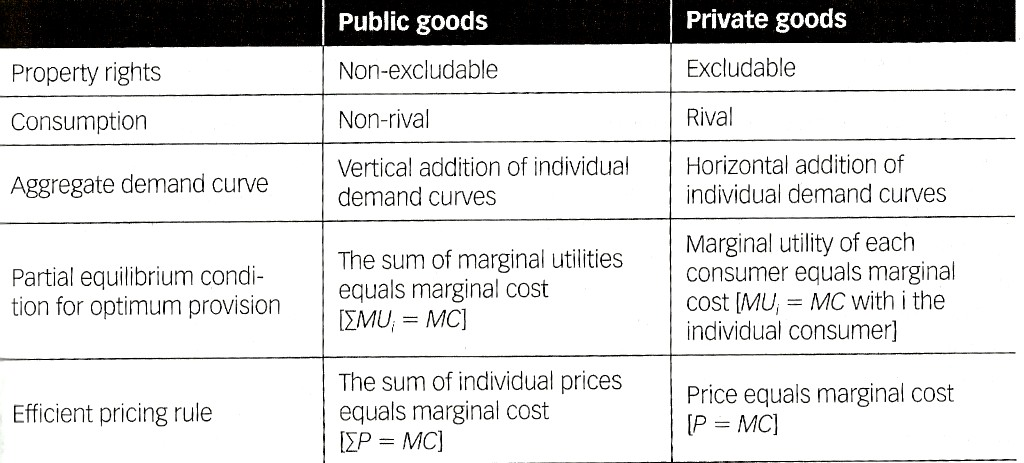
\includegraphics[scale=0.3]{./imgs/31t.jpg}

\sh{Explain why it is necessary for government to provide public goods.}
\ra Due to Excludability and rivalry.
\ra Market will not provide public goods, efficient pricing implies zero price (MC = P = 0)
\ra Consumers cannot be excluded once the good or service is available in the market. (Pareto-inefficient to exclude, therefore not possible to determine equilibrium price.)
\ra Leads to free riding (understating preferences) and under provision of public goods. 
\ra Government can improve ineffective markets but still not optimal. 
\ra Optimal provision of a public good requires prices discrimination due to summing individual prices. However government does not have the knowledge to do this therefore, they force consumers to pay a tax price, but is difficult to determine due to lack of preferences.
\ra Governments therefore levy a compulsory tax, forcing consumers to revel their preferences
\ra Public goods can be provided by private sector through public finance (has pros and cons). (textbooks, medicine, dams, university)
\ra Goods supplied will depend on the political process
\ra Is part of privatisation debate

\sh{Explain what mixed and merit goods and services are and debate whether the public or private sector should provide them.}
\ra Posses both private and public goods characteristics.
\ra Mixed goods are a Grey area
\ra Two classes
\rn{1} Non-rival, excludable mixed goods and services. Non-rivalry prevents market supply because both MC = 0 and charging a price leads to Pareto-efficiency. Toll-road. DSTV.
\rn{2} Rival, non-excludable mixed goods and services. Example is a congested road. MC increases with usage. Could charge a price but it is not possible to apply exclusion principle due to cost constraints. 
\ra Technology can influence non-excludability
\ra Merit goods are mixed or private goods which are politically sensitive goods usually provided for b y the national budget. They confer external benefits on the broader community. Education and health.
\ra Merits goods lead to prohibition such as drugs and smoking, controversial due to interest groups and their paternalistic nature.
\ra Government could supply alone such as healthcare or Private sector can supply such as toll roads and TV. 
\ra Most mixed goods tend to be supplied by both public and private sector, such as public and private educational institutions.

\sh{"The market is unable to provide national defence efficiently." Discuss this statement critically.}
\ra Defense is a public good
\ra Non-Rivalry and because indivisible goods 
\ra Non-excludability on cost grounds is most common as cannot exclude unwilling to pay citizens. Free-rider problem.
\ra Criticism technological add cost-effective to privatise

\sh{Distinguish between different categories of positive and negative externalities.}
\ra Positive if actions of consumer/producer confer a benefit to external parties
\ra Negative if actions of consumer/producer impose a cost to external parties
\ra Actions can be 
\rn{1} Technological: directly effect production/consumptions level 
\rn{2} Pecuniary: directly affect demand and supply, hence affect market prices. Can be argued that there is no net effect on society, as its a is a transfer from one owner to another.
\ra The they drive a wedge between private and social costs/benefits.
\ra Social costs/benefits = sums of private and external costs/benefit.
\ra Supply Side:
\quad 1) Negative. MEC > 0 and MSC > MPC.
\quad 2) Positive. MEC < 0 and MSC < MPC. 
\ra Demand Side:
\quad 1) Positive. MEB > 0 and MSB > MPB. 
\quad 2) Negative. MEB < 0 and MSB < MPB.
 
\sh{Negative production externalities, how government can promote allocative efficiency?}
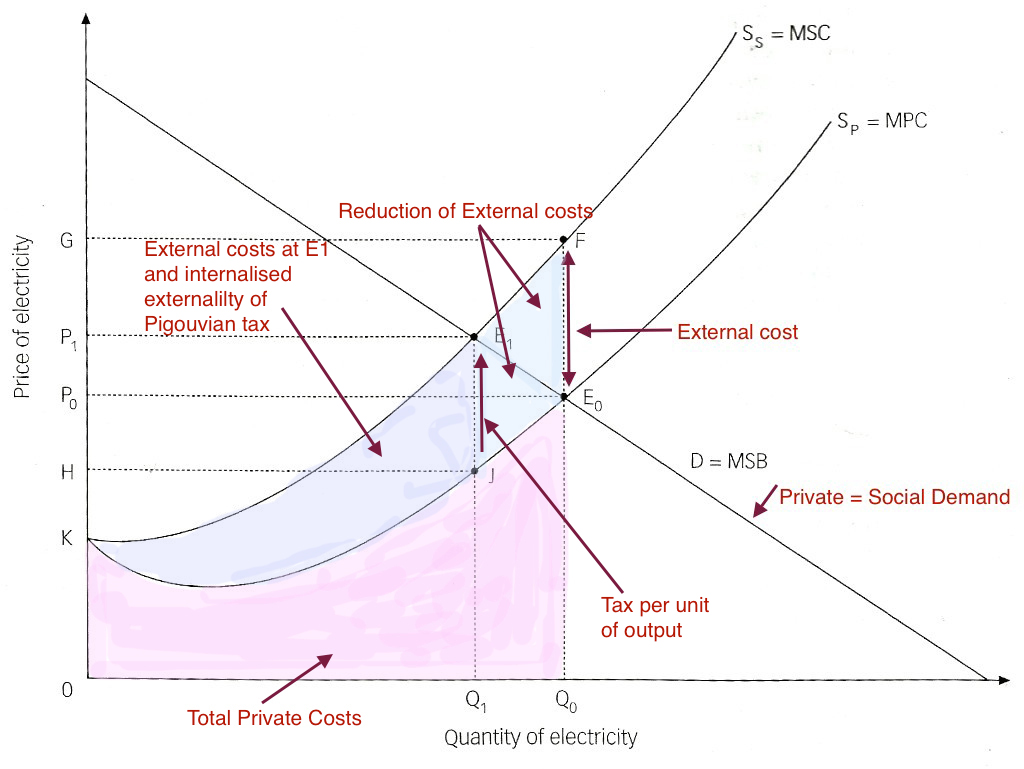
\includegraphics[scale=0.3]{./imgs/33.jpg}
\ra e.g. Coal fired power station polluting nearby farmer's water.
\ra Normal market situation equilibrium at $E_0$ with $Q= 0Q_1$ and $P_e=0P_0 $ 
\ra $E_0$ does not account for external cost of pollution $S_s=MSC$.
\ra $Q_0E_0 + E_0F = Q_0F$
\ra Total private costs are $0Q_0E_0K$ and total external costs are $KE_0F$. 
\ra If externalities are taken into account equilibrium is at $E_1$ with decreased quantity $0Q_1$ and and higher price $0P_1$.
\ra A negative production externality causes inefficiency in the form of over-provision and under-pricing of goods.
\ra In moving from $E_0$ to $E_1$ the externality was reduced to $KJ_E1$.
\ra Consumers are prepared to except the reduced negative externality because of the benefits of the provided good.
\ra The opposite of a positive production externality implies the MSC lies below the MPC, e.g. bee keeping.

\sh{Positive externalities, how government can promote allocative efficiency?}
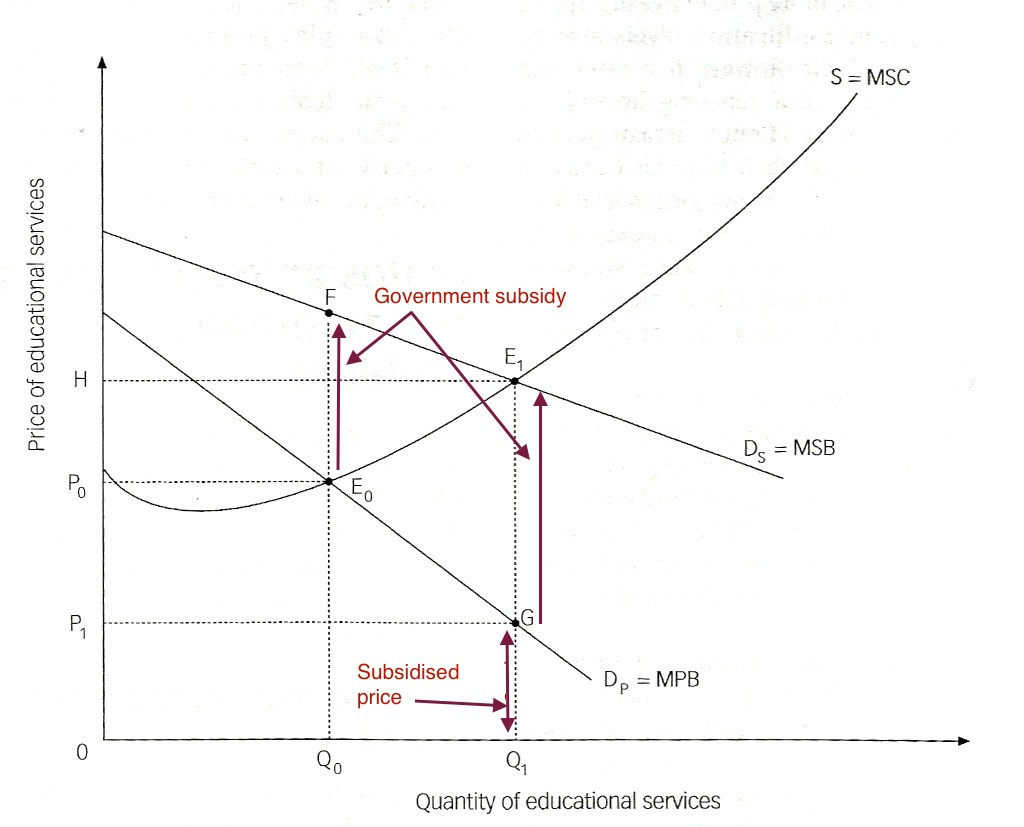
\includegraphics[scale=0.3]{./imgs/34.jpg}
\ra e.g. Education.
\ra MPB is skill accumulated, expected higher earnings and enjoyment.
\ra Equilibrium is at point $E_0$
\ra MSB is positive externalities from education, such as dissemination of information to the benefit of others free of charge for their increased welfare. Higher education leads to reduced social ills and relieves pressure on government finances.
\ra MSB lies above the MPB and equilibrium is at $E_1$ with higher price $0H$ and increased quantity $0Q_1$
\ra Competitive markets therefore under-provided and under-price goads and services.
\ra Pigouvian subsidy raises the effective price and increases quantity supplied.
\ra Opposite case of negative benefit with MSB lying below MPB, e.g. playing loud music.


\sh{Different policy options available to correct externalities.}
\ra 4 Interventions
\rn{1a} Pigouvian taxes for negative externalities 
\rna Attempt to internalise negative externality by increasing the producers MPC to the level of the MSC, by an ad valorem tax on the price.
\rna A tax of $E_0F$ shifts $S_p$ to $S_s$ and the price to $F$, but with supply exceeding demand at point $F$ equilibrium settles at $E_1$. 
\rna An efficient Pigouvian tax must be equivalent to marginal external cost at the $E_1$ which is $JE_1$.
\rna The internalised externality is $JKE_1$ and reduction in externality is $JE_0FE_1$
\rna Emission fee or congestion tax is levied on the externality itself. If unit tax exceeded unit cost of reducing emissions, then producers would reduce output or use new technology to reduce emissions unit MC of reductions equals unit tax, e.g. congestion charging for cars in London.
\rn{1b} Pigouvian subsidies for positive externalities 
\rna If government subsidises education by $E_0F$ it would shift $D_p$ to $D_s$
\rna At $F$ price plus subsidy induces a positive supply response and equilibrium will be at $E_1$
\rna Consumers would pay $Q_1G$ with subsidy $GE_1$ and suppliers receive $Q_1E_1$
\rna The subsidy must equal the MSB to provided an optimal output. 
\rna $E_1$ is has larger quantity of education by lower per unit price $Q_1G$.
\ra Pigouvian taxes are subject to informational constraints, as it unrealistically assumes authorities are perfectly informed about the size of the externality or the supply and demand curves.,
\ra Pigouvian taxes can have perverse result such as in alcohol consumption.
\rn{2} Regulation
\rn{3} Creation of markets
\rn{4} Establishment of property rights.

\sh{Should Pigouvian taxes be used to internalise the negative external effects of tobacco and alcohol consumption}
\ra Tobacco and alcohol have huge externalities for the broader community.
\ra Tobacco smoking is major cause of heart disease and lung cancer and require expensive medical treatment paid for my tax payers.
\ra For tobacco SA attempts to reduce the externality by using excise taxes, prohibiting smoking in public spaces, ban on adversing and promotion and restrictions on tar and nicotine levels.
\ra An unintended effect of a tax hike on excise duties is smuggling.
\ra Smuggling is a large portion of the market, SA has cheaper substitute from neighbouring countries. The tobacco is usually of lower quality thereby increasing the externality.
\ra If the reduction in the externality from a tax hike is less the increase in smuggling, the tax could lead to an increase in the externality.
\ra A similar substitution effect happens for alcohol.
\ra Cheaper substitutes are of lower quality and increase the externality.
\ra  If the reduction alcohol usage a tax hike is less the increase in cheaper substitutes, then the tax could lead to an increase in the externality.
\ra Another unintended effect is the adverse impact of the tax hikes on income distribution.
\ra In patriarchal household the male head would continue to consume and the same quantities thereby reducing the income available for other necessities, and thereby the whole household is worse off than before the tax hike or the male head might change to cheaper more toxic substitutes with similar negative externalities.

\h{Study Unit 3}

\sh{Explain the social cost of a monopoly.}
{\bf Benchmark model}
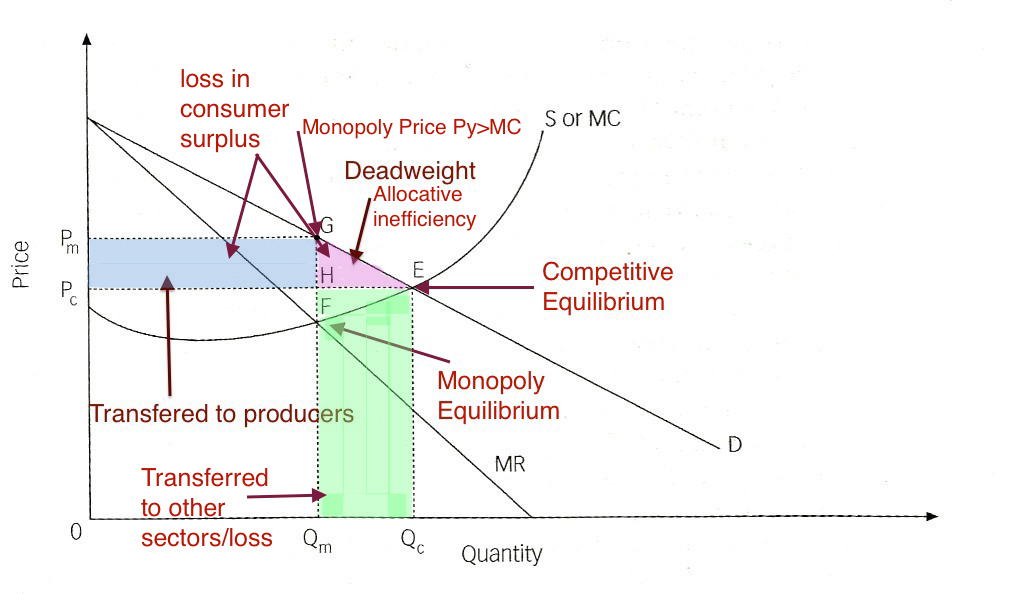
\includegraphics[scale=0.4]{./imgs/41.jpg}
\ra MC represents MC of monopoly firm only. MC represent sum of MC curves for individual firms
\ra Perfect competition equilibrium at E, Quantity = $0Q_c$, Price = $0P_c$, and 
\ra Under monopoly equilibrium at F where  MC=MR, Smaller Quantity = $Q_m$, Higher Price = $0P_m$ 
\ra Loss of consumer surplus $P_CP_MGE$,  transfer of consumer surplus to producers $P_mGHP_c$ and dead-weight welfare loss $GHE$. $HEQ_cQ_m$ also a social cost, due to time lags in transferring to other sectors.
\vspace{6pt}
{\bf Two-sector model}
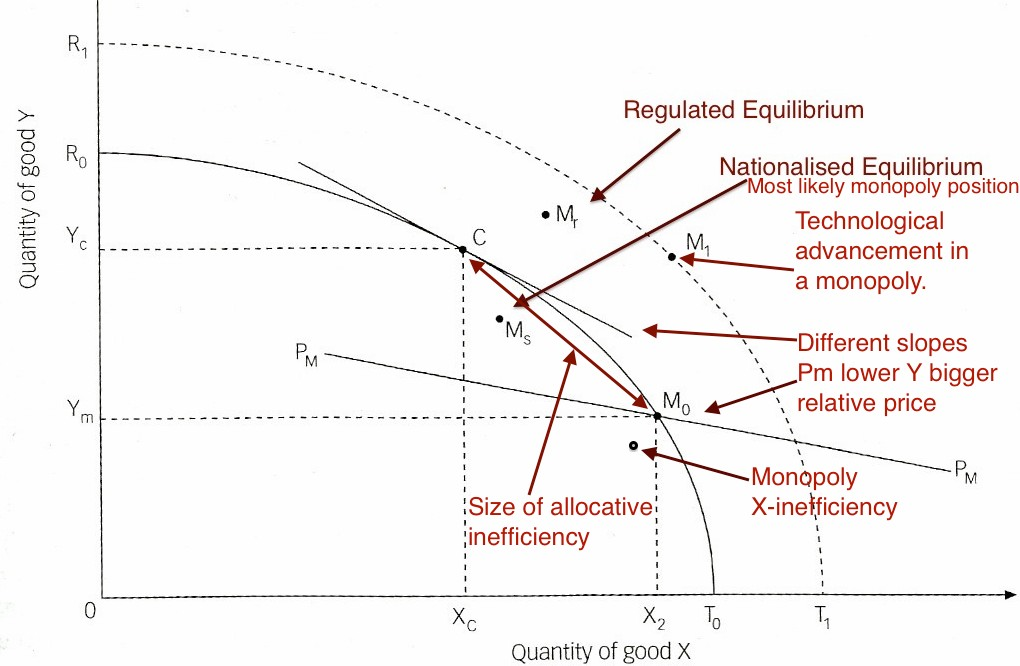
\includegraphics[scale=0.4]{./imgs/42.jpg}
\ra Given a monopoly then $P_y > MC_y$ and $P_x=MC_x$
\ra Because $MRPT_{xy} = \frac{MC_x}{MC_y} = \frac{P_x}{P_Y}$ then under monopoly $MRPT_{xy} > \frac{P_x}{P_Y}$ 
\ra Pareto inefficient, difference in slope between point C on $R_0T_0$ and commodity price line $P_MP_M$ passing through point $M_0$.
\ra Monopoly Lowers output of good Y and raise its relative price.
\ra Difference between $M_0$ and C is degree of allocative inefficiency
\ra X-inefficiency: Monopoly firms lack incentive to maintain high productivity, under utilise resources. point below $M_0$ 
\ra Monopolists are in a better position to achieve technological advancement. Shifts PPC to $R_1T_1$ and equilibrium to $M_1$
\ra Deregulation to improve allocative efficiency/X-efficiency and move towards point $C$ however might entail loss of profits to monopolists and loss of technological innovation, therefore gain will depend on if efficiency increases are bigger than losses. 

\sh{Government actions to improve efficiency}
\rn{1} Deregulation. Often monopolies are caused by government (liquor licences, patent right,  statutory bodies). Deregulation attempt to promote competitive by removing theses regulatory barriers.
\rn{2} Do nothing. In time, obstacles preventing entry to the market may disappear. In the long run, the demand curve could shift as a result of changing patterns in taste, rising incomes and the development of substitutes. Other firms might enters the contestable monopolist market resulting in a more competitive equilibrium.
\rn{3} Tax policy. Movement imposes taxes to tax away excess profits, however it does not improve the allocation of resources. 
\rn{4} Price control. Government can reduce the price of the monopolist by fixing it at $P=MC$. Excess profit is reduced and the socially efficient output level is achieved, however it is difficult to measure marginal costs and if the price is fixed to low will lead to black market prices and further measures.

\sh{Natural monopoly - Decreasing cost case}
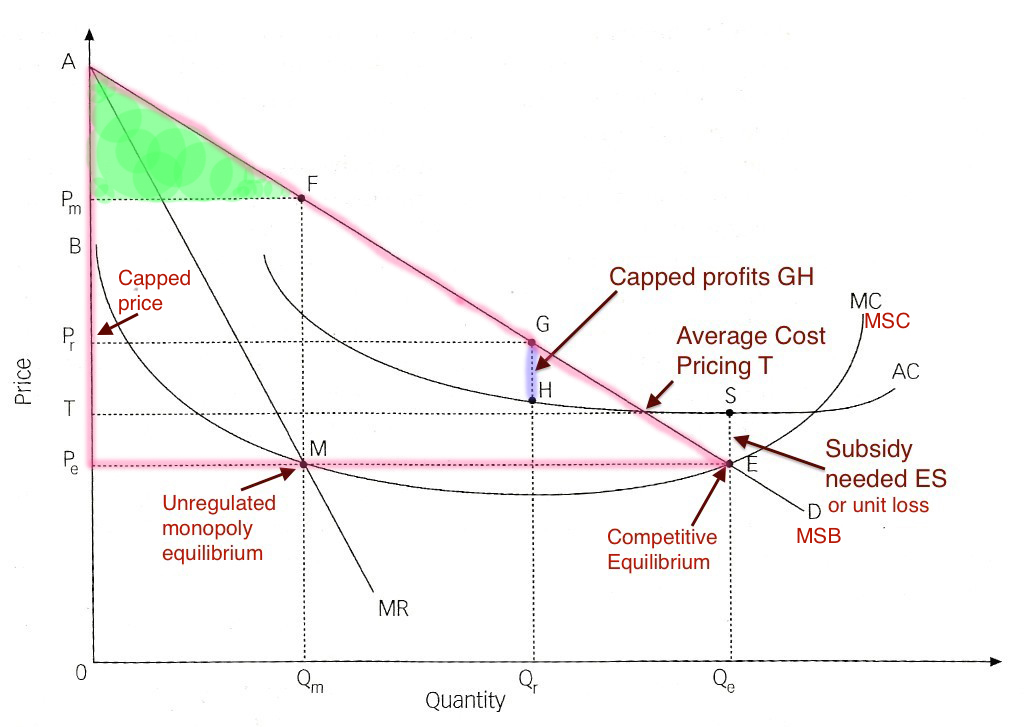
\includegraphics[scale=0.35]{./imgs/43.jpg}
\ra Large capital outlays that give rise to economies of scale over the entire range of its output.
\ra Minimum cost of production level sufficient to supply whole market therefore only one firm can effectively operate in the market
\ra Public utilities, like rail, water, postal.
\ra Increasing returns to scale means the long-term AC diminishes as output increase, MC curve lies below AC curve.
\ra Perfect competitive market equilibrium at E, with increasing returns to scale, industry will make a unit loss $ES$ and individual firms will eventually close till a natural monopoly emerges.
\ra Unregulated equilibrium would be at $M$, price $OP_m$ exceeds socially efficient price $0P_e$ and quantity $0Q_m$ is smaller than Pareto-efficient $0Q_e$. (to little output at higher price therefore welfare loss)
\ra Consumer surplus $AFP_m < AEP_e$

{\bf Government Intervention}
\ra if D=MSB and MC=MSC then MSB > MSC therefore a need to increase quantity and lower price to confer pecuniary externalities.
\rn{1} Government can start-up or take ownership and apply MC pricing at E and then subsidies loss ES. Results in x-inefficient point $M_S$ on PPC model due to taxes need to pay for subsidy.
\rn{2} If government borrowed money it would increase the interest and crowd out private spending in the rest of the economy. $M_s$ on PPC.
\rn{3} Regulation: Capping profit at maximum allowed $GH$ or capping price at $0P_r$.
\rna Profit capping is less popular because of cost padding.
\rna Price capping also administratively burdensome because of growth forecasts of input costs and demand
\rna Sliding scale, combines both capping options, when profits reach a certain level the price is adjusted down.
\rna Both consumers and producers benefit from efficiency gains an outward shift of PPC to point $M_r$
\rna Regulations strikes balance between need for economic growth  (outward shift of PPC) and the need for higher allocative efficiency.
\rna Pro's and con's below.
\rn{4} Deregulation not an option.
\ra Financing government investment such as social infrastructure from privation gains, can only be justified if the resources are applied more efficiently that it would be by the private sector,  otherwise net welfare would decrease. (Private sector could have spent funds on other things besides buying state assets.

\sh{ Discuss the case for and against privatisation.}
\ra Use PPC figure of two sector model.
{\bf For}
\ra Reduce excess burden caused by tax financing.
\ra Borrowing to nationalise increases interest rates and crowds out private investment. 
\ra Using taxes to nationalise creates tax wedge and loss in welfare
\ra Private monopolies are more X-efficient 
\ra Government monopolies are X-inefficient and rely on the never ending resources of the state.
\ra Private monopolies have more incentive to initiate and implementation cost-saving innovation due to shareholders or takeovers.
\ra Sales of state assets can be used to redeem public debt or boost investment (if applied more effectively than private sector).
\ra Can regulated to avoid abnormal profits for efficiency reasons and protect consumers/producers
\ra Nationalisation has fallen out of favour
\ra Would boost economic growth
\ra Lessen government expenditure and interest payments
\ra Broaden the tax base and enable tax cuts.
\ra Expected improvement in efficiency depends on if goods are prices at full cost or subjected to competitive market.

{\bf Against}
\ra Government monopolies are needed to create and confer pecuniary externalities on other industries. 
\ra Government monopolies have an allocative advantage
\ra Regulation is administratively burdensome.
\ra Can result in job losses
\ra Worsening of wealth distribution.
\ra Sale of assets may accrue to those that are already rich (worse distribution of wealth)
\ra Sales are once off i.e. Selling the family silver.
\ra Public enterprise can support socially important activities by cross-subsidisation
\ra Production still occurs under non-competitive conditions. (Private managers might not be more efficient.
\ra Anticipated efficiency from privatisation might not come to fruition.

%%%%%%%%%%%%%%%%%%%%%%%%%%%%%%%%%%%%%%%
\h{Study Unit 4}

\sh{Distinguish between Pareto and Bergson criteria for a redistribution of income}
\ra The Pareto criterion implies that a policy induced change is justified only if it improves the well-being of at least one person without harming any other. (Entitlement theory, other Pareto criteria)
\ra The Bergson criterion is broader and allows for a welfare improvement even if one or more individuals are harmed. (Welfare economics)

\sh{Critically discuss Nozicks entitlement theory and relevance to SA.}
{\bf 3 Principles of just distribution}
\ra  1: Justice in acquisition. Individual are entitled to acquire things that do not belong to others, or does not place others in a worse position, 
\ra  2: Justice in transfer. Material things can be transferred on a voluntary basis.
\ra  3: Rectifications of injustice. Redistribution of wealth justified only if one or both of the first two principles has been violated. This principle is the justification for redistribution.
\ra In terms of these principles a distribution is just if it arises from a prior just distribution by just means.
\ra Difficulty in identifying how far back to go to first injustice.
\ra Nozick's principle where applied in SA by TRC which had a limited focus from March 1960 to December 1993. The TRC was established to bring about national unity and develop human rights. It concluded that apartheid era victims were to be paid reparations.
\ra Two tasks need to be done:
\rn{1} A thought analysis of historical events giving rise to violation of first two principles.
\rn{2} An analysis of the distributional patterns that would have emerged in the absence of injustice.
\ra Requires large amounts of historical data, which are subject to human prejudice.
\ra Only allows for redistribution of capital goods and property not labour income which is an inalienable right and cannot be redistributed due to equity or efficiency reasons. Contentious but does simplify application.
\ra Pareto implications if A enriched himself at B's expense and against B's will then A should give back to B and place both parties in the same position before the injustice.

\sh{Explain under what conditions redistribution will be Pareto optimal.}
\ra {\bf Justified in terms of the theory of externalities.}
\ra The poor cause negative externalities on the rich, therefore the rich are prepared to transfer part of their income to the poor to reduce negative externalities.
\ra No single rich person can do, therefore government action required
\ra Government policy such as transfer payments, basic services, security systems, education subsidies, taxes on crimes (fines).
\ra {\bf Insurance motive }
\ra Tax payments viewed as relatively inexpensive means of insuring against future loss of income or ill-health. 
\ra Viewed as a cheaper alternative to private insurance.
\ra Not charity but a quid pro quo principle. Rich expect same benefits if they were poor.
\ra {\bf Altruism} see next.

\sh{Altruistic behaviour as a Pareto-based justification for income redistribution}
\ra Concerned and generous individuals experience a net increase in their utility from a policy that taxes their income and redistributes in favour of another non-altruistic individual.
\ra Therefore a movement along the PPC would improve the welfare of both individuals.
\ra Implies existence of external effects.
\ra $U_a=f(M_a,U_b(M_b))=g(M_a,M_b)$. $a$ derives utility from own income and $b$'s level of utility. $b$ only from their own income.
\ra $A$ derives utility not only from their own income but also from individual $B$'s utility level.
\ra Pareto efficient redistribution condition. $A$'s utility from $B$'s higher income ($g'(M_b) > 0$) must exceed the decrease in $A$'s utility from $A$'s lower income ($g'(M_a) < 0$). i.e. A net increase in $A$'s welfare.
\ra Giving to beggars or donating to charity are examples.
\ra Redistribution by the fiscal process is involuntary, but tax payers have the same altruistic tendencies.

\sh{Cardinal welfare function or additive social welfare function.}
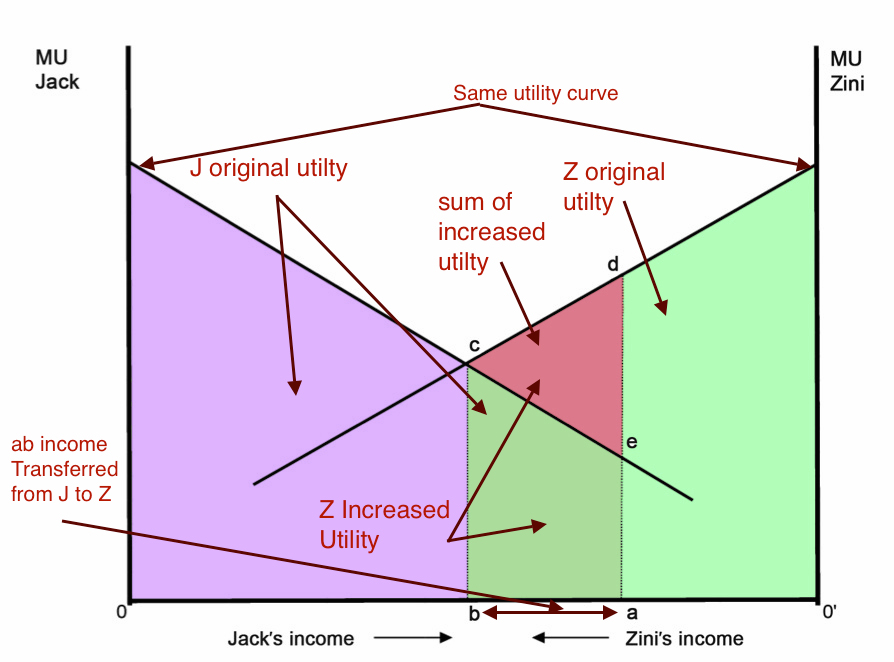
\includegraphics[scale=0.3]{./imgs/51.jpg}
\ra Social welfare function, community welfare defined in terms of all the individual utilities.
\ra $W=U_a+U_b + \dots$
\ra It also allows for Pareto criterion, when $W$ increases if $U_a$ and/or $U_b$ increase, or if the decrease in one utility is less than an increase in another utility.
\ra Example R10 utility for rich versus poor, therefore giving R10 to poor is greater utility than the lost utility to rich.. 
\ra Allows for redistribution of income.
\ra {\bf Assumptions}: 
\rn{1} Utility diminishes as income increases. Difficult prove that marginal utility from extra income decrease.
\rn{2} It assumes individual utility functions are identical and only depend on income.  Impossible to determine validity of incidental utility function as they can't be measured objectively.
\rn{3} The total amount of income is fixed. Taxes and subsidies changes the work ethic decreasing total income. Savings would decline as well reducing total income.
\ra Welfare will be maximised when MU's are equal at point C.

\sh{Ordinal or generalised welfare function}
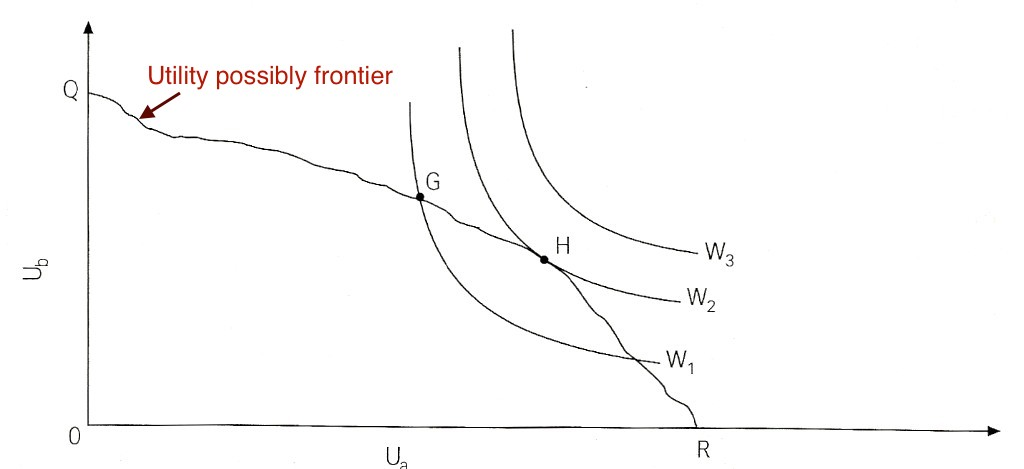
\includegraphics[scale=0.25]{./imgs/52.jpg}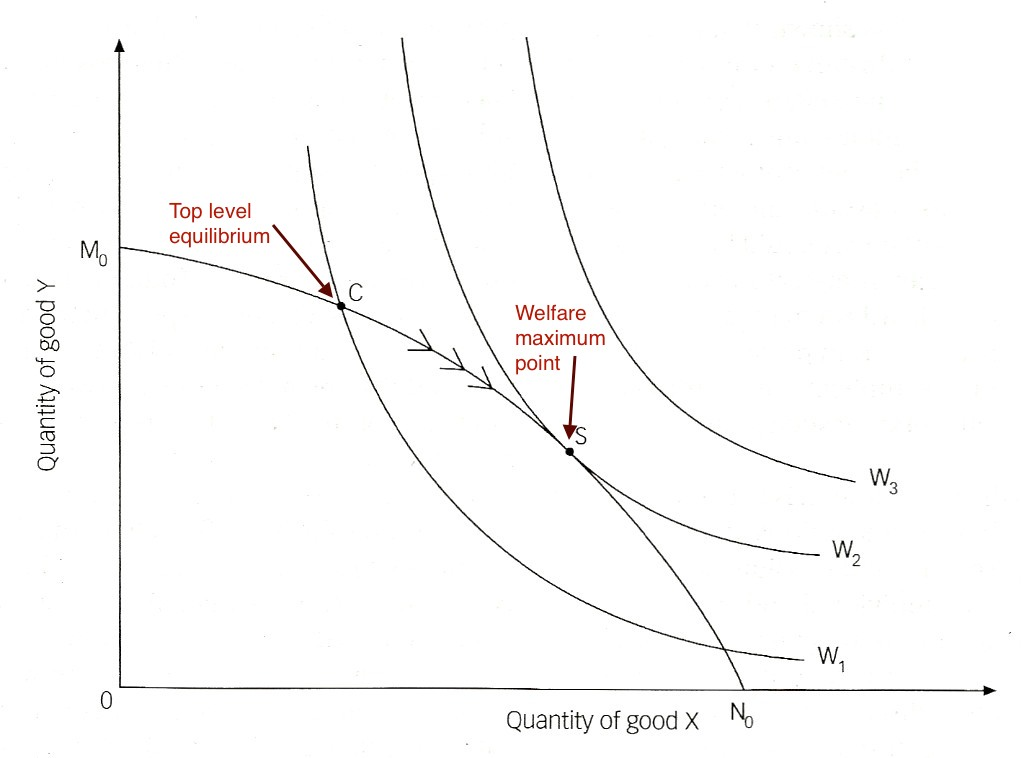
\includegraphics[scale=0.25]{./imgs/54.jpg}
\ra Generalised welfare function. $W=W(U_a,U_b)$ where $U_a=U_a(X_a,Y_a)$
\ra Function is ordinal in nature and does away with the assumption of measurability.
\ra Function produces community indifference curves. $W_1, \dots$, (convex to origin, cannot intersect, diminishing MRS). Value judgement based.
\ra The commodity based social welfare function $W=V(X,Y)$ where $X=X_a+X_b$. These are superimposed on the PPC top find the optimal welfare position point $S$.
\ra All points on PPC are Pareto optimal, but each point reflects a different income distribution. A person who owned most capital and had preference for good Y would leave competitive equilibrium at point $C$. 
\ra Government intervention is needed to move economy closer to S by taxes fro instance. Which would reduce utilities of certain individuals, Bergson Criterion.
{\bf Assumptions:}
\ra Community is able to choose between points (public choice theory)
\ra Choosing a particular point implies a value judgement about the relative worthiness of two individuals $a$ and $b$, and yet the same social welfare. Also implies a judgement on the worthiness of two sectors, given that $U_a$, might favour commodity $X$. 

\sh{Pareto optimality is a necessary but not a sufficient condition for a welfare maximum}
\ra Discuss ordinal functions and movement along PPC from top-level equilibrium to welfare maximum.
\ra Top-level competitive equilibrium is only a necessary condition for social welfare but not a sufficient condition.
\ra In the two sector model all points along the PPC are Pareto-efficient
\ra Each point corresponds to a particular distribution of income and one individual is in a better position than another in terms of income at different points.
\ra Therefore a competitive economy producing the output at the optimal point would not not necessarily also yield the most preferred distribution of income.
\ra Redistribution is Pareto inefficient because if one persons position is improved it would negatively affect another persons position.
\ra Discuss ordinal welfare use PPC.

\sh{Policies aimed at promoting equity can contribute to inefficiency}
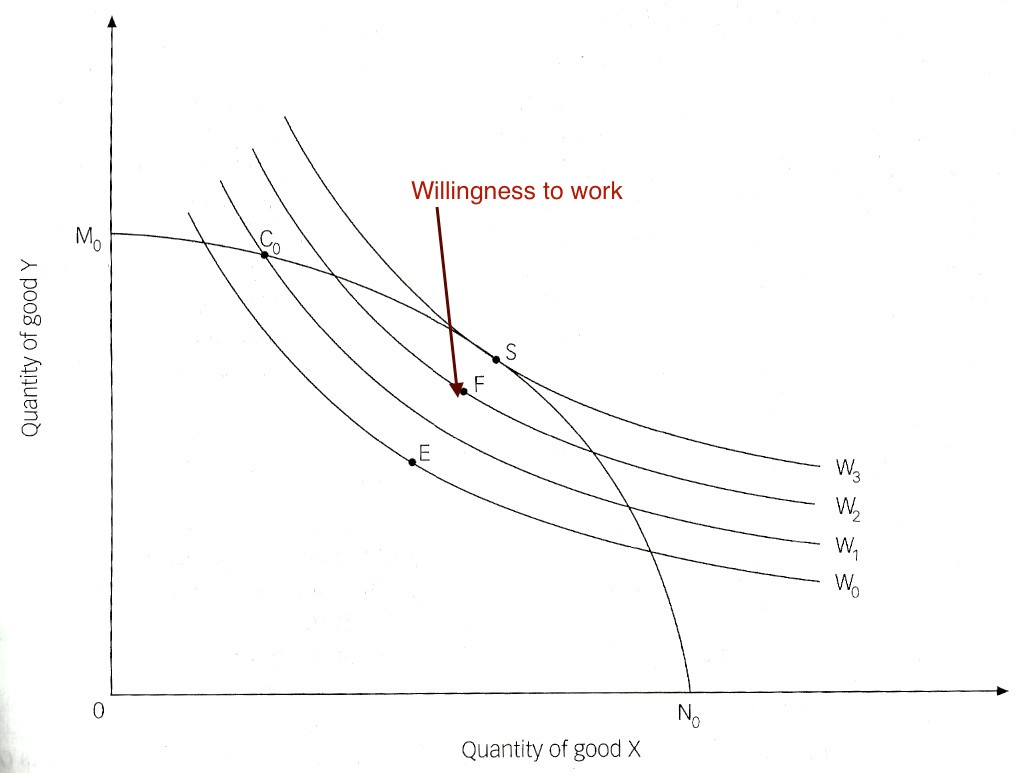
\includegraphics[scale=0.3]{./imgs/55.jpg}
\rn{1} Affects the willingness to work.
\rna Above a certain level increased taxes have a negative effect on the willingness to work.
\rna In moving economy from top-level equilibrium $C_0$ to welfare maximum $S$ by taxing industry Y or subsiding industry X, then with a disincentive to work effect, productivity falls and the economy ends up at point $F$
\rna point $F$ is a higher welfare level. 
\rna A point $F$ there is conflict between equity and efficiency and a hence a trade-off due to the higher welfare.
\rna A more pronounced effect could leave economy at point $E$ and a lower welfare level.
\rn{2} Dynamics consequences of taxing rich and subsidising poor.
\rna A tax would limit savings and investment hence limit growth. This could keep the economy at point $S$, $F$ or $E$, 
\rna In the absence of the tax the economy could have grown and the PPC would have naturally shifted.
\rna Large wealth and income inequalities have negative externalities, in the absence of corrective redistribution policies investor could consider the economy as unstable and negatively affect savings and investment. Therefore doing nothing could result in a point inside the PPC.

%%%%%%%%%%%%%%%%%%%%%%%%%%%%%%%%%%%%%%%
\h{Study Unit 5}
\sh{Give an overview of how public choices are made in the political market.}
\ra Suppliers (politicians and bureaucrats) and Demanders (voters)
\ra Voters use voting systems to signal wishes
\ra Others means include protesting and lobbying
\ra 3 Voting systems.
\rn{1} Unanimity voting
\rna Each member or representatives group within a community must support a proposal before it becomes the collective decision. 
\rna Leads to Pareto-optimal outcomes.
\rna An example is a Rawlsian welfare function. If people are risk averse and they vote from behind a veil of ignorance, voters will attempt to maximise the utility of the person with the lowest utility. Application for present day SA in its current empowerment charters.Are voters so risk adverse that they unwilling to take chances or would they accept a small probability of being poor for a large probability of being rich.
\rna Problems: Time consuming and costly to win support of all, May lead to tyranny of the minority, with minority holding the majority to ransom.
\rn{2} Simple majority voting.
\rna Gives each person one vote and the proposal needs 50\% plus one vote to be accepted.
\rna Two process used to determine preferences are: {\bf Direct democracy} such as referendums and {\bf indirect democracy} such as representative democracy.
\rna Median voter model: Under a majority voting system in which preferences are not extreme, the median voters preferred option will win due to its is minimum welfare loss for the whole group.
\rna Advantages: Less costly and less time consuming than unanimity. Less likely a minority can prevent a majority from getting proposals accepted.
\rna Arrows impossibility theorem. Not always possible to derive a logically consistent set of individual preferences on the basis of an ethical acceptable social choice rule.
\rna Disadvantages: 1) Outcomes are logically inconsistent when preferences are extreme. 2) Outcomes depend on the order of voting 3) There is agenda manipulation 4) Intensities of preferences are ignored (Can be overcome with point voting and vote trading) 5) Tyranny of the majority over the minority due to winner takes all.
\rn{3} Optimal voting majority
\rna To minimise external costs (vote goes against a group of voters) and decision-making costs (persuasion costs) the optimal voting majority for each issue would differ. There would be different voting rules for different issues.
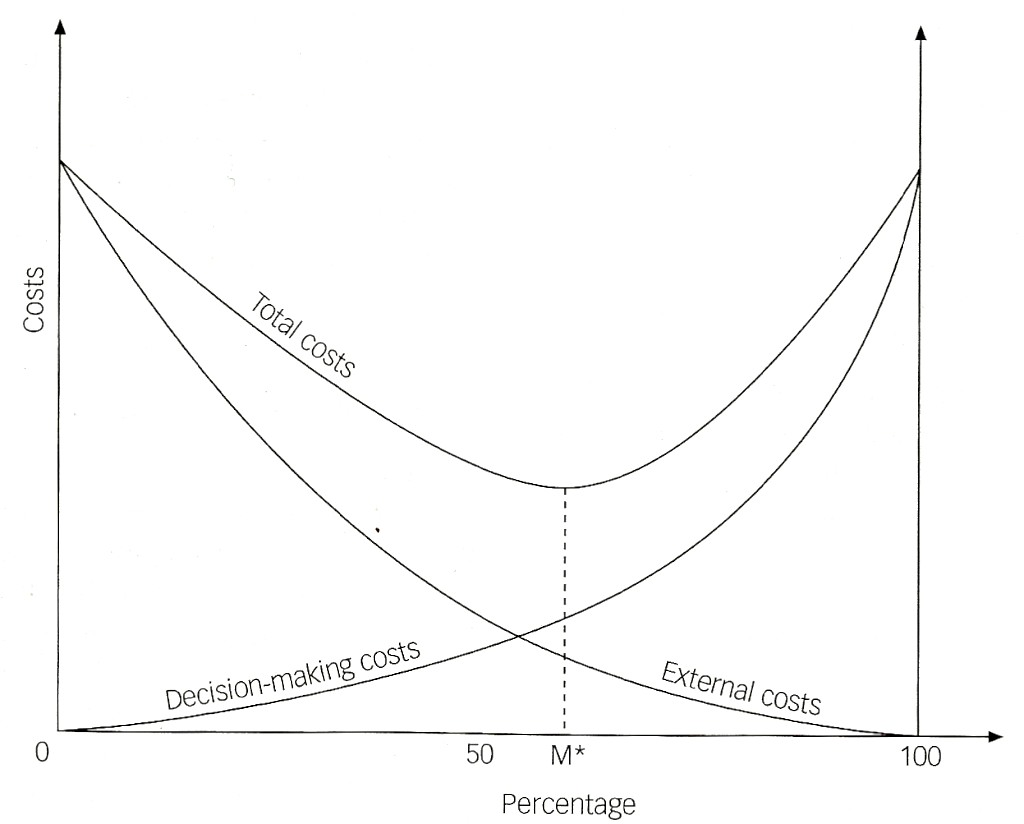
\includegraphics[scale=0.3]{./imgs/61.jpg}

\sh{Politicians and government failure}
\ra Viewed as entrepreneurs who engage in vote maximising strategies in order to secure and retain political office.
\ra Voters are rational ignorant of what politicians stand for and lack incentive to acquire necessary information.
\ra Politicians are elected on the basis of a package of policies and only have to please a majority of voters on each policy issue.
\ra Above gives rise to implicit logrolling coalitions favouring special interest legislation, in which politicians understate the real costs of their policies to appeal to the majority.
\ra Politician therefore create a preponderance of special interest legislation producing a variety of relatively unpopular public goods.
\ra They create an aggregate oversupply of public goods.
\ra Can be dealt with by constitutional reform by limiting the proportion of scarce resources expended on public goods.

\sh{Bureaucrats government failure}
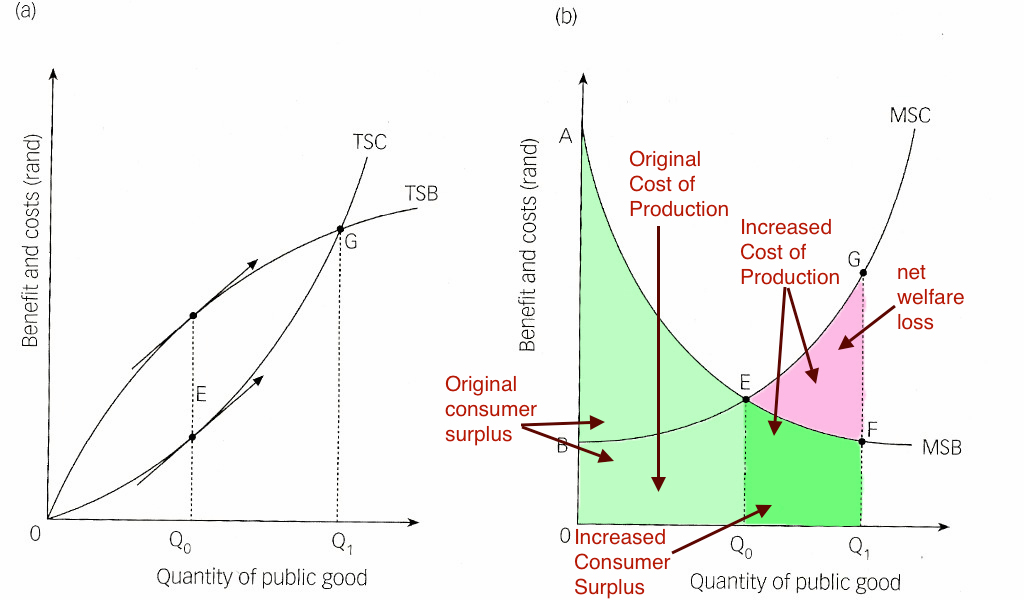
\includegraphics[scale=0.35]{./imgs/62.jpg}
\ra Rational responses from utility-maximising civil servants to the incentives presented by politicians and institutional structures.
\ra Since higher salaries, more power and prestige and other favourable attributes are positively related to department size, bureaucrats have an incentive to maximise their budgets, as opposed to cutting cost to maximise profits of private firms.
\ra TSC: total social costs rise increasingly faster while TSB: total social benefits rise decreasingly slower as output expands.
\ra Social optimal output $0Q_0$ where $MSB=MSC$ parallel tangents. 
\ra A budget maxing bureaucratic would attempt to justify output $Q_1$ where the $TSB=TSC$ where $MSC$ exceeds $MSB$ by $FG$
\ra Detail coloured areas.
\ra The increase total cost exceeds the increase in total benefits with a resulting new welfare loss.
\ra A principle agent problem. Bureaucrats have greater incentive to increase spending than taxpayers have to reduce taxes.
\ra Problems with Niskanen model:
\rn{1} Unrealistic to assume that politicians and tax-payers are at the mercy of bureaucrats.
\rn{2} Budgetary procedures have become more transparent.
\rn{3} Salaries and perks are usually not linked to budget size.

\sh{Rent-seeking and corruption}
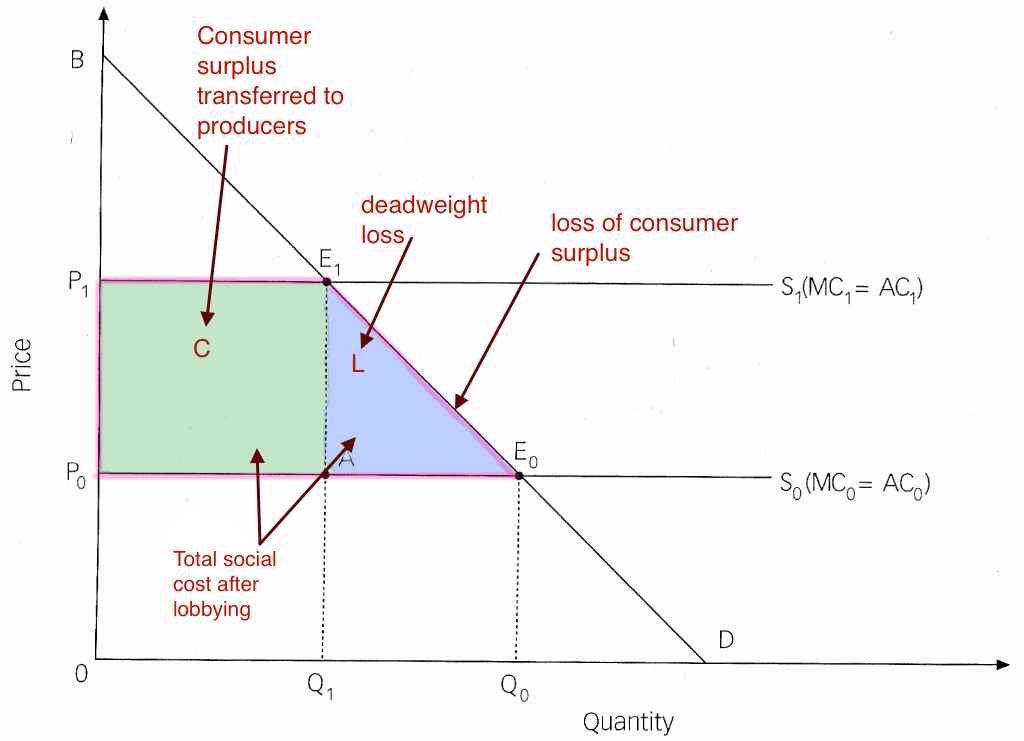
\includegraphics[scale=0.35]{./imgs/63.jpg}
\ra Governments interventionist roles serves as an incentive to interest groups or engage in rent-seeking
\ra Government intervenes by tendering provision of public goods and services and by regulating goods and service not in the public interest.
\ra Economic rent is define as that part of the reward accruing to resource owners over and above the payment they would receive in alternative employment. Similar to monopoly profit and cannot be competed away.
\ra A competitive market would ensure a re-allocation of resources to eroded the rent.
\ra Governments create artificial rent, such as government protected monopolies or regulations.
\ra Equilibrium at $E_0$ with price etc.
\ra If government restricts output to to $0Q_1$ prices increase to $0P_1$ and loss of consumer surplus $C$.
\ra $C$ is a costless transfer to producers while $L$ is the deadweight welfare loss.
\ra $C$ is available for suppliers to boost their profits and would incur addition costs to capture this rent. With 2 possibilities.
\rn{1} Participating suppliers. 
\rna Additional lobbying cost would shift $S_0$ to $S_1$ where all rent would have been dissipated.
\rna This results in suppliers transferring part of their own resources away from productive activities in favour of non-productive rent seeking actives.
\rna The total social cost would be $C+L$.
\rn{2} Concerned citizens
\rna In this case additional cost will be external to the suppliers and $C$ will be a transfer to producers who would receive additional income to save or spend.
\ra Rent seeking is a social waste.
\ra Creation of rents creates potential for corruption, such as bribes or kickbacks. 
\ra Corruption is illegal and producers would do so only if the net benefit exceeded the cost of the bribe, and being detected and punished.
\ra Corruption is widespread indicating inadequate legal system and the need for trust worthy and honest individuals.

\h{Study Unit 6}

{\Large\bf Macro Models}
\sh{Wagner and the stages-of-development approach}
\ra How government expenditure tends to increase when a country develops from a subsistence or additional economy to an industrialised economy. 
\ra First Stage: Create law and order, legal and administrative institutions needed to cut costs of doing business, start investment providing roads, railways, harbours. Mainly capital expenditure.
\ra Middles stages: Continued government investment expenditure. Private sector investment increase due to positive pecuniary externalities from previous government investment, however causes market failures (monopoly pricing, high-density living conditions) that government must increase spending on to address.
\ra Last Stages. Development capital as percentage of GDP decrease. Increased expenditure on eduction, health, welfare and social security increases due to high-income elasticity of demand for them. Therefore a continuous increase ion government expenditure. 
\ra SA followed early and middles stages (capital expenditure) however decreased public investment is not a sign that SA in last stages.
\ra Some rural areas have not entered the first stages of development.

\sh{Peacock and Wisemans displacement effect}
\ra Government expenditure depends broadly on revenues raised by tax, and government would continue to increase their expenditures and expanding their role provided the economy continued to grow through industrialisation. However there would be resistance to higher taxes from voters and government expenditure would therefore only grow when strictly necessary.
\ra Social upheavals or financial crises necessitate rapid increase in government expenditure and therefore higher taxes are needed.
\ra Displacement affect is then certain government expenditures (war related expenditures) displacing private expenditures as well as other government expenditures. 
\ra Tax payers will accept higher taxes during times of social upheavals and financial crises. 
\ra Increased government expenditure should decrease to pre-crises however it is most likely to remain at post-crises levels due to tax payer ambivalence.
\ra In SA apartheid era military/social protection build-up due to social unrest, including increased education expenditure due to school unrest
\ra Displacement pressures were dampened somewhat by spending on social services. 

\sh{The Melzter-Richard hypothesis}
\ra A general equilibrium model in which the majority voting determines the magnitude of income distribution and the size of government expenditure.
\ra Increase in government expenditure was due to an extension of the suffrage which brings about a change in the median voter.
\ra Median voter is important in two-party democracy as they choose who will win and politicians seek their support.           
\ra  If the income of the median voter lies below the average income there will be pressure for redistribution. To gain the support of the median voter parties will emphasise redistributive policies that could result in higher taxes and higher expenditure on social services, with the median voter effectively determining the tax rate.
\ra There is not unlimited redistribution because of the disincentive effects of higher taxes leading to people working less and a smaller scope for redistribution. 
\ra In SA did not happen after 1994 with introduction of poor median voter, because of 1) previous expenditure to avoid social upheaval, or 2) does not apply, or 3) fiscal restraint in macro-economic stability forced reallocation.

\vspace{12pt}
{\Large\bf Micro Models}
\sh{Baumol's unbalanced productivity growth}
\ra Government expenditure may increase disproportionately due to the price of inputs used by the public sector relative to those employed in the private sector.
\ra Baumol divided the economy into two sectors.
\rn{1} Progressive Sector
\rna Characterised by technological progressive activities such as innovation, capital formation and economies of scale, contributing to a rise in output.
\rna Important feature is a cumulative increase in the productivity of labour justifying increases in wages and salary.
\rna Labour is only one of the inputs in the production process
\rn{2} Non-progressive sector.
\rna Inherent characteristics permit only sporadic changes in productivity.
\rna Labour is often the end product
\rna Usually consists of services that also constitute a large component of the public sector. Such as education and law and order.
\rna Technological change does not have such an important effect on productivity.
\ra Example, comparing labour in manufacturing versus highly talented labour such as a pianist. There is limited room for productivity increases in a piano concert.
\ra There cannot be to large wage or salaries difference between the two sectors otherwise labour would leave the non-progressive sector for the progressive. This raises the relative costs of the non-progressive sector as there is no accompanying productivity increases.
\ra The cost of even a constant level of activity from the government would be expected to grow.
\ra Also a larger portion of labour would need to be employed in the non-progressive sector to maintain production, thereby have a negative effect on the economy.
\ra A critique is the underestimated opportunities for technological advancement in the public sector like computerisation.
\ra In SA government expenditure corresponds with Baumol's unbalanced productivity growth hypotheses,  however no empirical test have been conducted.

\sh{Brown and Jackson's microeconomic model}
\ra  Developed a microeconomic model to derive the levels of public provided goods and services by taking the preferences, income and tax rate of the median voter (determinants of demand) and the costs of the goods and services.
\ra The perceived lack of increased service levels from increase government expenditure can be explained by changes in the service environment.
\ra Example increased crime, increased policing same perceived levels of service. Without increased expenditure service would seen to be deteriorating.
\ra Changes in the size and density of the population and its age structure will also influence the service environment.
\rna Increases in the population will lead to either higher levels of expenditure or a drop in standards.
\rna If the relative price of services decreases (economies of scale from increased tax base) it may be an incentive for government to increase provision of services and increase expenditure.
\rna Increased density would increase governments costs
\rna The fight against HIV/Aids, malaria and tuberculosis increase government expenditure.
\ra A good or service is of a superior quality if it requires more inputs in it production than a similar service and therefore increases in quality would put pressure on government expenditure.
\ra On the whole a relevant model for studying government expenditure in African countries.

\sh{Role of politicians, bureaucrats and interest groups}
\ra \note{incomplete} 

\sh{Government and the economy: long term effects}
\ra NGT \note{incomplete} 

\ra Crowding in \note{incomplete} 
\ra Crowding out \note{incomplete} 

\h{Study Unit 7}

\sh{Distinguish between primary and secondary income, and importance of secondary income}
\ra Primary income or personal income. Actual value of income received in cash or kind by individuals, including value of subsistence agricultural.
\ra Secondary income: Primary income less direct taxation (only taxation which can be assigned with reasonable accuracy) = disposable income + value of government services consumed.
\ra $Y_s=Y_p-T_d+G_s$ \quad $G_s=$ social expenditure (only category reliably attributable to households with any certainty.
\ra Given the high degree of racial inequality of primary incomes in SA it would be best to study the impact of reducing inequality by study secondary income.

\sh{Explain the balanced budget incidence.}
\ra $G_S-T_d$ = fiscal incidence (net result of tax and expenditure incidence). Linked to determining the normative question of fairness and burdens of $G_s$ and $T$.
\ra Balanced budget incidence: combined effect of government spending and taxes levied. Distributional impact of a tax depends not only on the incidence of the tax itself but also on how the government spends the proceeds from the tax.
\ra Government spending on defense has different distributional impact compared to financing old-age pensions.
\ra The balanced budget incidence ignores the distributional impact of policies on primary incomes. Primary income distribution already incorporates an element of fiscal incidence, double counting should be therefore avoided. Example company tax has already influenced personal income by reducing the after-tax income to shareholders, or VAT's reduction of consumer purchasing power.

\sh{List the ways in which government can influence income distribution}
\ra The government budget embodies the fiscal measures of redistribution. It influences income distribution by determining government expenditure and how the expenditure is financed (taxes and loans) including long-term distribution of human capital that fundamentally determines the distribution of incomes.
{\bf Mainly Affecting Primary income}
\ra Rule-maker, rules of the competitive markets.
\ra Controller of prices and wages in markets
\ra Market operator (employer of labour, size and nature of purchasing)
\ra Long term influence (industrial decentralisation, impact of taxes on capital intensity of production)
{\bf Affecting Secondary income (fiscal redistributor}
\ra As Taxer, supplier of public goods, welfare transfers
\ra Redistributor of assets  

\sh{Describe the perceived distributional impact of different taxes.}
\ra In terms of statutory incidence the most progressive taxes are income taxes, with a possibility of a negative income tax (transfer) for low levels of income. An alternative to means tested transfers.
\ra Wealth taxes are progressive
\ra Selected excise taxes are too seen as progressive
\ra Most indirect taxes are seen as regressive and can be reduced through zero rating certain food items, however erodes tax base and increaser the complexity of administration.

\sh{Analyse the economic effects of a subsidy and show how it can create an excess burden.}
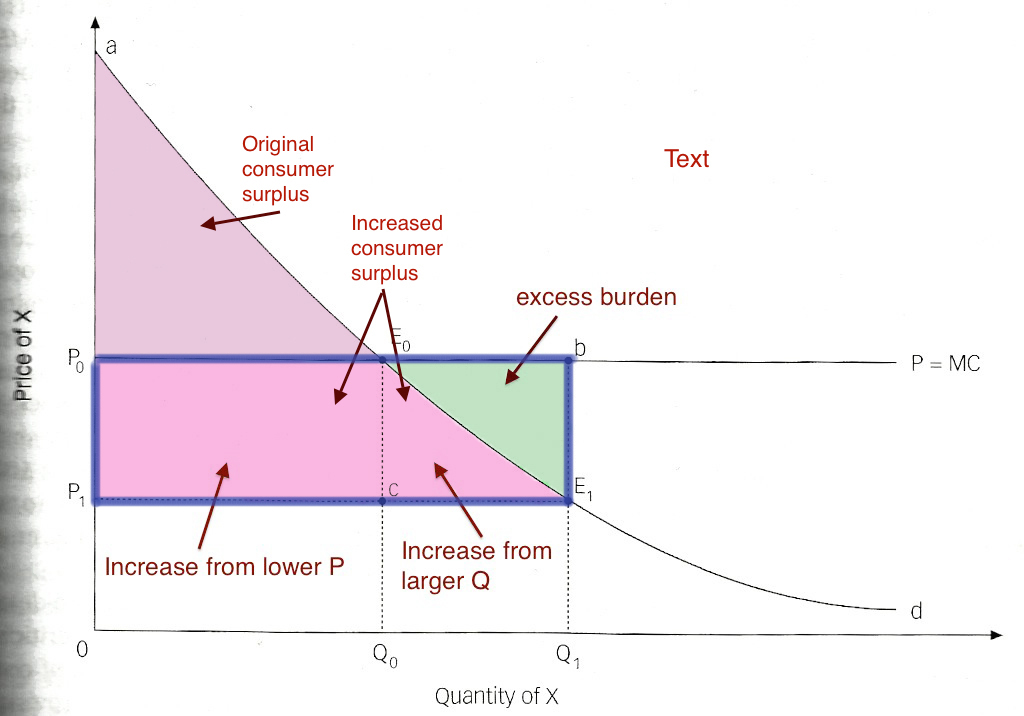
\includegraphics[scale=0.3]{./imgs/82.jpg}
\ra The costs of a subsidy are larger than its benefits, leaving an excess burden due to economic inefficiencies.
\ra Assuming constant production costs, after the full benefit of a subsidy has been passed on to consumers, the price would decrease from $P_0$ to $P_1$ and quantity increases from $Q_0$ to $Q_1$ and an increase consumer surplus from $aP_0E_0$ to $aP_1E_1$
\ra Cost of subsidy is $P_0bE_1P_1$ leaving dead weight welfare loss $E_0bE_1$
\ra Subsidies interfere with consumer choice and lead to socially suboptimal outcome.

\sh{Explain how government can redistribute assets through indirect means.}
\ra Direct interventions require large degree of coercion and are only common in post-revolution situations, such as nationalisation or land redistribution without full compensation. Has limited application in market based economies. 
\ra Indirect asset transfers at full compensation are slower and have a high cost in terms of reduced social spending. (e.g Land-reform versus Health expenditure)
\ra Income transfers can increase wealth through savings.

\sh{List the characteristics of social spending in developing countries.}
\ra In industrialised countries emphasis has shifted from indirect (infrastructure, defense investment) to more direct satisfaction (education, health), which required increased taxation and hence growing tax resistance.
\ra In developing countries social spending is constrained by limited fiscal resources.
\ra Given the limited resourced, social spending ratios have risen nonetheless since WW2, to much higher levels than today's industrial countries at a similar stage in development.
\ra Have been biased towards urban populations, mainly benefiting non-poor.
\ra Spending targeted higher-eduction rather than primary, hospitals rather than primary health care facilities, which again benefit privileged.
\ra Congo: Pubic expenditure largely devoted to inflated public sector, similarly in Swaziland.
\ra In developing countries social security has been neglected, with education expenditure dominating.

\sh{Effect of a cash transfer, funded by income tax, on work effort}
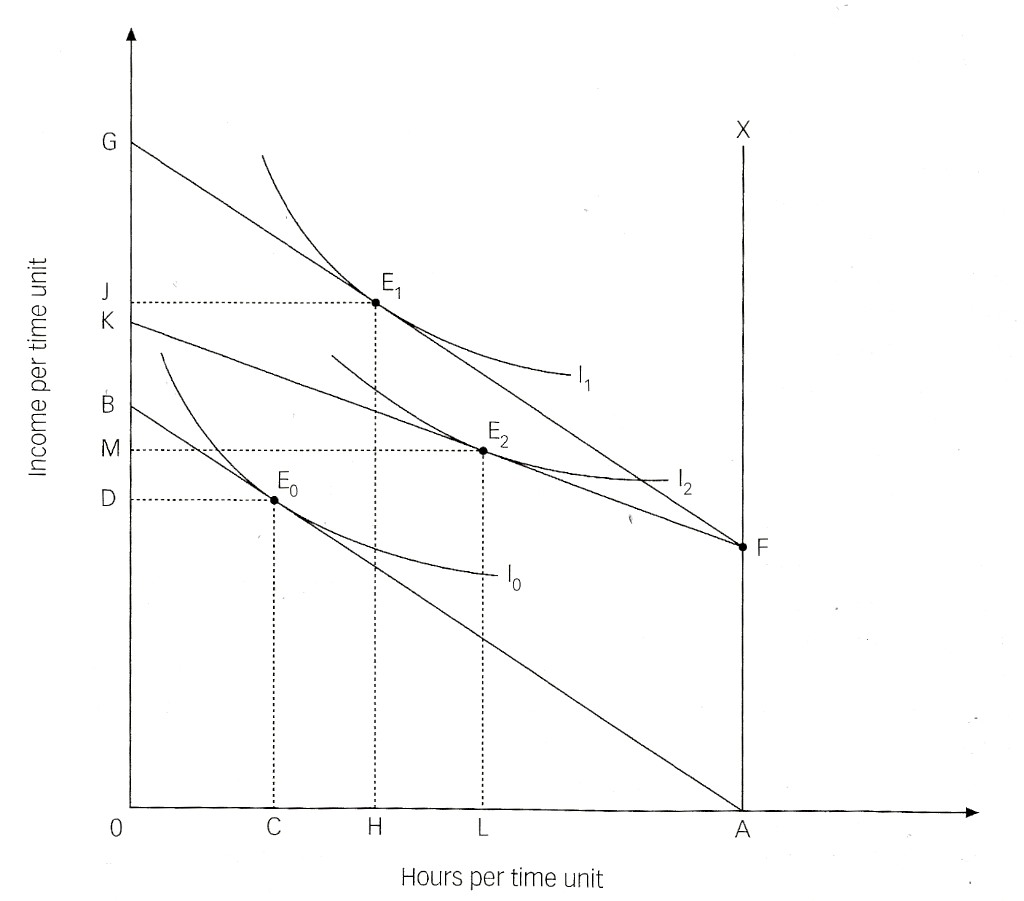
\includegraphics[scale=0.3]{./imgs/83.jpg} 
\ra $0A$ worker hours are allocated to either work or leisure
\ra Vertical line $AX$ signifies that time endowment is fixed at all income levels
\ra $AB$ show workers combined budget/time constraints, where sacrifice leisure implies higher income.
\ra Initially equilibrium is at $E_0$ given indifference curve $I_0$, working $AC$ hours and continuing $)D$ goods. (no savings, value of goods = income earn)
\ra If G provides income transfer, budget line shifts $GH$, with equilibrium at $E_1$ and higher indifference curve $I_1$. Consumption of both leisure and goods has increased. Higher welfare but works fewer hours due to income effect.
\ra If income tax is imposed to finance cash transfer, reducing opportunity cost of leisure, budget line swivels to $FK$ and work effort is further reduced to$AL$
\ra The combined effect of a cash transfer and taxation reduced work effort by 1) negative income effect 2) negative net effect $HL$ of taxation.
\ra Policies need to ensure combinations leas to minimal reduction in work effort. Social old-age pensions have provided no incentive to work less.
\vspace{6pt}
{\bf Poverty trap:} certain regulations or tax systems make it unattractive for people to increase their private income beyond certain levels as this leads to reduction ins sate benefits,.


\sh{Explain by means of a graph the incidence of a housing subsidy when both the demand and supply curves are moderately elastic.}
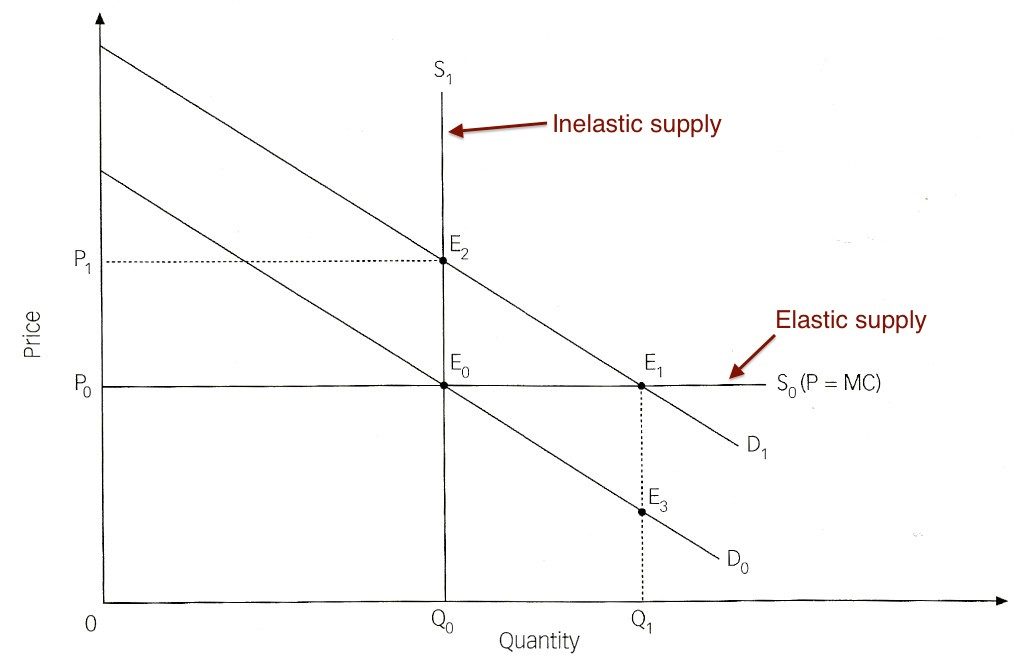
\includegraphics[scale=0.3]{./imgs/84.jpg} 
\ra The case for G intervention is based on needs  argument and existence of externalities (enhance return on non-residential physical investment and social invest like education.)
{\bf Perfectly price-elastic supply $S_0$}
\ra Initial equilibrium at $E_0$ with ${P-0}$ and ${Q_0}$
\ra Housing subsidy increases consumer purchasing power and shift demand curve upwards to ${D_1}$.
\ra Equilibrium is now at ${E_1}$ and price ${P_0}$ and increased quantity ${Q_1}$, buyers enjoy the full befits of the subsidy and no shifting occurs
{\bf Perfectly price-inelastic supply $S_0$}
\ra A subsidy only results in a price increase to ${P_1}$ and new equilibrium at ${E_2}$. 
\ra Only benefits capitals of exiting homeowners, completely cancelling benefit of subsidy to buyers,
{\bf Moderate elastic supply.}
\ra Some benefit will accrue to exiting how owners through increased demand and higher prices. 
\ra Some benefit will accrues to the intended beneficiaries through increase processing power (reduction of costs) and acceleration of housing supply..
\ra Increased prices means some benefits accrue to the construction industry and in general equilibrium context to owners of the factors of production (labour and capital)


\ra Incomes to low to even afford a small rudimentary house.
\ra providing a proper house to everyone is unaffordable therefore incremental housing provision.
\ra \note{add more}
 
%%%%%%%%%%%%%%%%%%%%%%%%%%%%%%%%%%%%%%%
\h{Study Unit 8}

\sh{List and describe the sources of government revenue}
\ra User charges: (benefit taxes), prices charged for the delivery of certain public goods and services. Set in the political market, and can only be levied if exclusion is possible. Toll roads, public swimming pools, ambulance service, university education.
\ra Administrative fees: similar to user charges but the service or benefit received is broad and imprecise. Business or television licenses, diamond export rights, fishing licences, vehicle license, traffic fines. Small source of revenue.
\ra Governments can borrow in domestic and foreign markets. Used to finance capital expenditure. Must be paid back at a later stage therefore a deferred tax. Should not be used for unproductive activities or consumption.
\ra Government induced inflation. (inflation tax) Financed in such as way as to increase the money supply thereby increasing the price level, and lowering the real value of government debt. Example a loan levy.

\sh{Define different categorises of taxes and give examples of each}
\ra Taxes are transfers of resources from persons or economic units to government and are compulsory and legally enforceable due to the free rider problem. 
\ra Not necessarily a direct connection between the taxes and the goods and services received such as cross subsidisation.

{\bf Types}
\rn{1} Taxes on income and profits. Important revenue source.
\rn{2} Taxes on payroll and workforce 
\rn{3} Taxes on property
\rn{4} Domestic taxes on goods and services. Important revenue source.
\rn{5} Taxes on international trade and transactions
\rn{6} Stamp duties and fees

\sh{Explain a progressive, proportional and regressive rate structure.}
\ra 3 taxes bases: income, wealth and consumption.
\ra Also a 4th tax on people, e.government lump sum tax per head (poll tax).
\ra Tax rate structure: amount of tax levied per unit of the tax base. 
\ra 2 ways to measure. 
\rn{1} Compare the average tax rate to the size or value of the tax base. 
\rn{2} Ratio of taxes paid to income base.
\ra 3 rate structures: 
\rn{1} Proportional, flat-rate. Average tax remains constant as tax base increases, or tax that generates the same proportion of revenue as income rises.
\rn{2} Progressive. Average tax rate increases as tax base increases. Generates increasing proportion of revenue as income rises.
\rn{3} Regressive. Average tax rate decreases as tax base increases. Generates a decreasing proportion of revenue as income rises.

\sh{Viewed as both a proportional tax and a regressive tax.}
\ra Compare rate per tax base versus rate per income base.

-------------------------
\ra General tax: (broad-based tax) tax entire tax base and allow no exemptions. Under certain assumptions similar to a head or lump sum tax and leaves relative prices unchanged. VAT with zero-ratings.
\ra Selective taxes: (narrow base tax) imposed on one or a few products. Distorts relative prices with tax wedge between before and after price. Violates Pareto efficiency conditions.
\ra Specific tax: Unit tax, a fixed amount per unit of the product. Excise duties per litre/box.           
\ra Ad valorem tax: Levied a percentage of price of a commodity. often imposed on luxuries. 15\% of car value.
\ra Direct tax: imposed directly on individuals and companies (personal income tax, company tax). Tax incidence cannot be shifted easily.
\ra Indirect tax: imposed on commodities like excise taxes and VAT. likely to be shifted tax incidence.
-------------------------

\sh{Indicate whether the following  taxes or levies are general or selective, specific or ad valorem, direct or indirect and explain your answer in each case: ?}
\rn{1} Personal income tax (Selective if includes exemptions otherwise general, its direct, ad valorem, percentage )
\rn{2} a 10\% tax on DVD players. (indirect, selective, ad valorem)
\rn{3} VAT (indirect, selective if includes exemptions otherwise general, ad valorem)
\rn{4} R1.02 per litre of fuel (indirect, selective, specific)
\rn{5} R200 levy on all economics students (selective, specific, direct (although could be seen as indirect as most parents would pay :))

\sh{Briefly describe the four properties of a "good tax"}
\ra Equity: Taxes should promote an equitable distribution of income. To determine fairness tax incidence should be examined.
\ra Economic efficiency: Taxes should be designed so that their distorting effects (excess burden) on the choices made by taxpayers is minimised.
\ra Administrative efficiency: Administration and compliance costs must be kept low.
\ra Flexibility: As economic circumstances change, taxes and tax rates need to adjust.


\sh{Benefit principle}
\ra Stipulates that the tax burden of government expenditure should be apportioned to taxpayers in accordance with the benefits each receives.
\ra Example a bridge used by some but financed by all.
\ra Forced carrying: someone being made to carry a heavier than normal burden.
\ra Tax morality would be undermined if tax payers did not benefit from a tax system.
\ra Advantages
\rn{1} Links expenditure side of the budget to the revenue side, and servers to regulate government expenditure.
\rn{2} Approximates allocative procedures of market behaviour, by assuming the role of prices and ensures that resources are efficiently allocated.
\ra Disadvantages
\rn{1} Scape for applying is restricted. Governments generally provide public goods and the benefits are generally non-excludable. policing for rich protection versus policing for vulnerable poor.
\rn{1} Takes existing distribution of income and wealth for granted. Distribution could be skewed towards the needs of the rich and therefore undermine the redistributive objectives of government resulting in conflicts. (e.g. old age pensioners financing themselves)
\ra  Befit taxes or user charges are levied on toll roads, museums entrance fees and license fees. There is a direct link between financing and the benefits. However the user charges prevent the poor from accessing these merit goods.  If the goods were to be provided free of charge and financed by general financing and the rich used them more, there would then be a redistribution from poor to rich. Can be offset by special reduction on elderly and children. 
\ra Earmarked taxes. Special funds or accounts for financing services that are indirectly related to the source of funds. E.g. fuel levies and unemployment insurance. Similar shortcomings to the benefit principle. Also earmarked taxes 1) affect the procedural fairness of the budgetary process by not having to complete with other departments 2) the accountability and efficient resource allocation is shifted to the managers of earmarked funds 3) complicates fiscal policy aimed at achieving macroeconomic objectives. The Katz Commission recommended against a proliferation of earmarked taxes especially those from VAT.

\sh{Ability-to-pay principle}
\ra Because the benefit principle cannot be applied to government provision of public goods, expenditure is therefore apportioned by the ability to pay principle. 
\ra It requires people with equal capacity to pay the same amount of tax (horizontal equity) and for people with great4er capacity to pay more (vertical equity)
\ra Horizontal equity requires similar tax treatment for people of similar economic circumstances. Same tax rats for same income groups.
\ra Vertical equity requires individual in different economic circumstances to be treated differently. Example the size of the different rats for the different income groups, high versus low. Involve and element of sacrifice and results in progressive tax structure.
\ra Requires public consensus on appropriate rate structure, measure, criterion, basis or indicators of ability to pay. Highly contentious issues because of subjective evaluations.
\ra Income. consumption, wealth and utility are general measures.
\ra Income is not perfect as it measure outcomes and not capacity, E.g a hard worker versus a lazy worker at the same wage rate means more ability to pay from hard worker.

\sh{Distinguish between statutory and economic incidence.}
\ra Only people (shareholders, workers, consumers) can bear the tax burden and not companies.
\ra Statutory incidence refers the legal liability to pay tax to revenue authorities.
\ra Economic incidence refers to who ultimately bears the tax burden. Excise tax on cigarette imports  can be shifted onto consumers with higher prices or onto workers with lower wages, it can also be avoided by reducing imports.

\sh{Balanced-budget incidence}
\ra The overall distributional effect of a tax and the spending financed by the tax is considered.
\ra Example income tax lowers real disposable income but tax spent on education and other public services raises real disposable income.  
\ra Advantage is it relates cost of spending programmes to those who pay.
\ra Disadvantage is linking a particular expenditure item to a tax source is almost impossible, because of the pooled tax revenue.

\sh{Differential tax incidence}
\ra Considers the distributional impact as one tax is substituted for another holding revenue and expenditure constant.
\ra The benchmark often used for comparison is a lump sum tax (head tax) that does not affect relative prices and economic behaviour.
\ra e.g. Substituting a lump sum tax on redheads for a excise tax on beer drinkers that generates the same revenue and then looking at its affects.

\sh{partial equilibrium analysis}
\ra If the prices change do not have  significant repercussions for other markers. Demand and supply are determined without any affect on other prices.
\ra less complex since ramifications of tax are not studied.
\ra Ideal for studying goods with few substitutes and complements and the secondary effects are considered small and uncertain and can be ignored.

\sh{General equilibrium analysis}
\ra Secondary effects of a tax are taken into account. e.g. Tax on butter raising the price of its substitute margarine. Demand and supply affect other prices.
\ra More suited for studying the incidence of a general sales tax, or a specific tax such as a fuel levy which impact the entire economy.
\ra Better than partial analysis because it considers relative prices changes.


\sh{Incidence of unit tax}
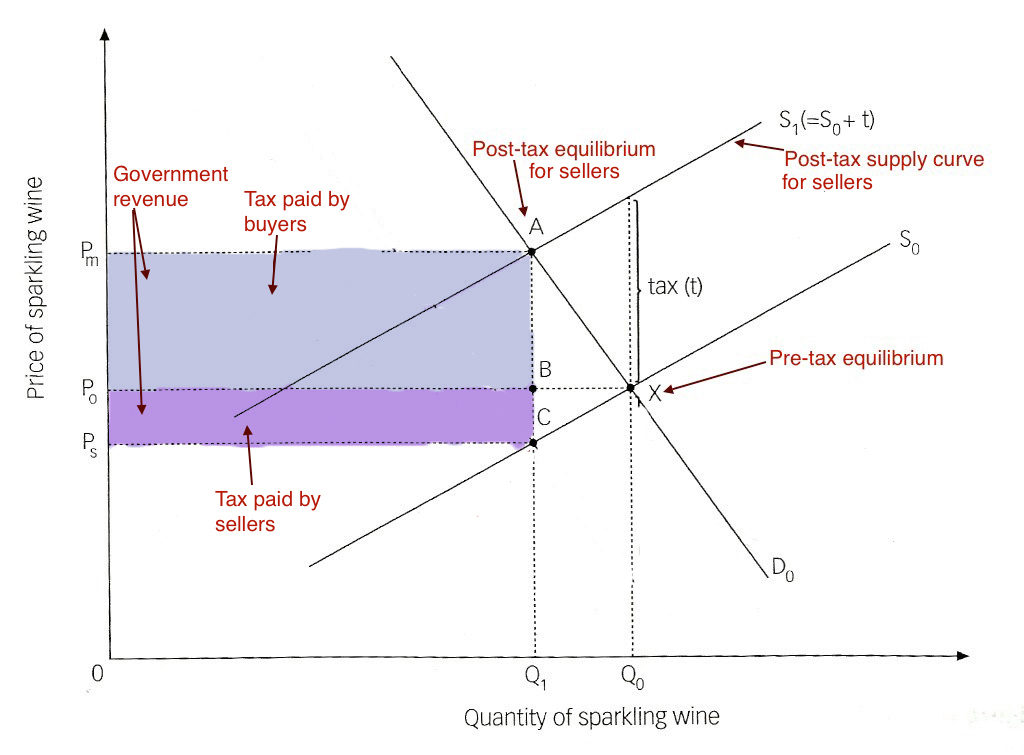
\includegraphics[scale=0.3]{./imgs/101.jpg} 
\ra State demand and supply give and before tax equilibrium details
\ra Suppose and excise tax per unit is applied. 
\rn{1} Statutory incidence is on sellers 
\rna To recover the full tax amount supply curve shifts up to $S_1$ with price $P_0+t$
\rna Supply curves are parallel because its a unit tax.
\rna New equilibrium at A, state details higher price $P_m$ and suppliers receive $P_m-t$
\rna Government tax revenue is $t \times 0Q_1 $, shaded blue
\rna Both buyers and sellers pay part of the prices and the tax incidence falls on both. Sellers do not pass on full tax burden to consumers.

\sh{Incidence of an ad valorem tax}
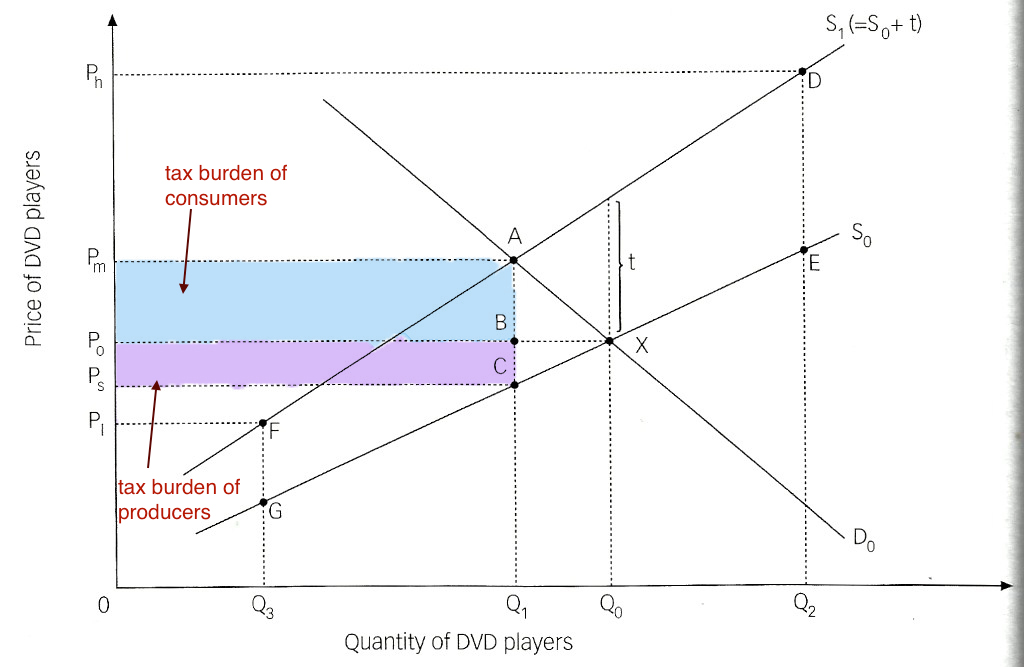
\includegraphics[scale=0.3]{./imgs/102.jpg}
\ra Different to unit tax case as supply curve swivels due to ad valorem tax, as the higher the price the greater the tax paid by producers.
\ra Therefore the supply curve will swivel upwards at the higher price and downward at the lower price.
\ra Same analysis has unit price from here.
\ra Ad valorem tax rate as ratio of tax to price is $\frac{AC}{AC_1}$ 

\sh{Incidence and pure monopoly}
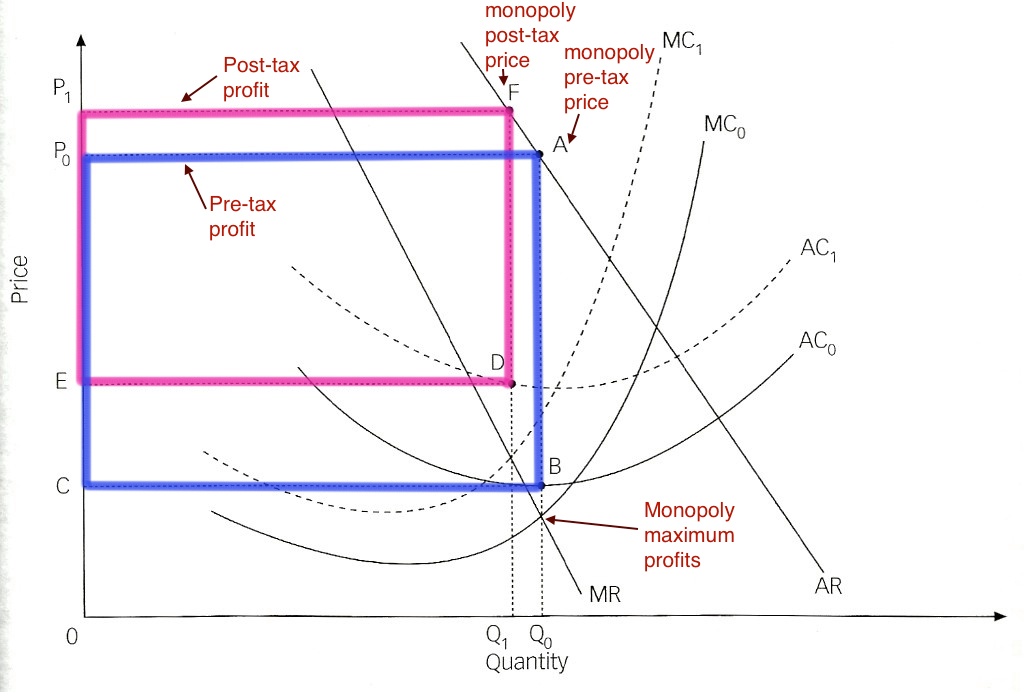
\includegraphics[scale=0.3]{./imgs/103.jpg}
\ra State pre-tax equilibrium $MR=MC$ with pre-tax profit
\ra After a unit tax average cost will rise and MC will rise as unit tax is a variable cost. Curves shift upward.
\ra Profit is not maximised at $Q_1$ and $P_1$
\ra Post-tax price is higher and the quantity is lower.
\ra Post-tax quantity is less and a pure monopolist does not shift the tax burden fully. If the firm was not maximising profits tax shifting could occur.
\ra Can also tax on Economic profits, the before tax profit area in figure. A tax of t will reduce economic profit by the tax amount. Neither the average or marginal cost curves will be affected and the monopolist will maximise profit as usual and the tax is fully borne by owners and the tax is not shifted.

\sh{Incidence and price elasticities of demand}
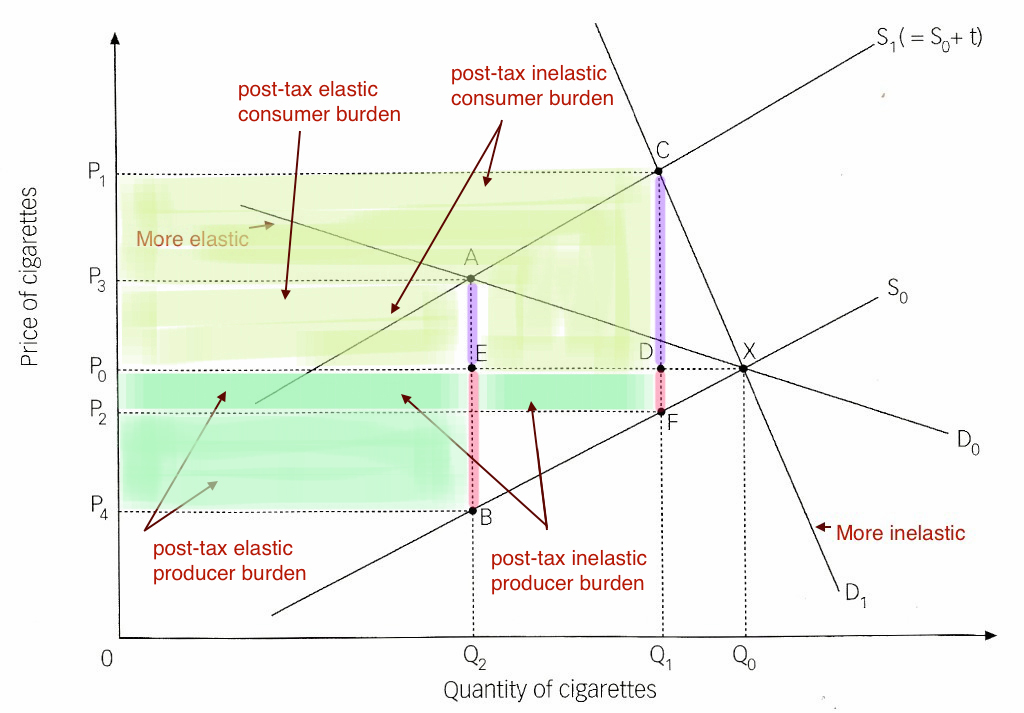
\includegraphics[scale=0.3]{./imgs/104.jpg}
\ra Two demands curve interesting at $X$ and supply curve plus price and quantity.
\ra Intersecting demand curves allow elasticity comparison. 
\ra Unit tax cause upward shift. 
\ra For inelastic demand details 
\ra For elastic demand details
\ra The more price elastic the demand for a product is (flat demand curves) the greater the proportion of the tax borne by producers.
\ra The more price inelastic the demand curve (upright) the greater the proportion of tax borne by consumers.

\sh{General equilibrium analysis of tax incidence.}
\ra Assumptions. 
\rn{1} 2 products (shoes, baskets), 2 factors of production (labour and capital)
\rn{2} Perfect mobility
\rn{3} Fixed supply of factors 
\rn{4} Shoes are capital intensive and baskets are labour intensive.
{\bf Selective tax on commodities}
\ra Say a tax is imposed on shoes, the prices of shoes increase relative to reed baskets.  
\ra Has two effects
\rn{1} Consumption side (uses)
\rna Demand for shoes decreases (movement along) and demand for baskets increases (right shift) and the price of baskets increases. 
\rna The tax causes an increase in the price of both products, incidence is spread to producers and consumer of the untaxed good too.
\rn{2} Production side (sources)
\rna Fewer shoes demand therefore fewer shoes produced, freeing up capital and labour for basket production. Because basket production is labour intensive not all capital is used and the price of capital will decrease and both sectors will use more capital, therefore the tax caused the returns on capital to decrease.
\rna The burden of the tax is also spread to the factor of production used most intensively in production of the taxed commodity.

{\bf General tax on commodities}
\ra A general tax is equivalent to a tax on income and the tax will be borne in proportion to the consumption or income of each member of the economy. 
\ra A general tax on commodities leaves relative prices unchanged including relative price on leisure.

\sh{Tax incidence and tax equity revisited}
\ra Luxuries, as income increases individual spend more (elastic demand). A statutory tax on buyers of leisures would be progressive. 
\ra Expenditure on necessities tends to fall as income increases and a tax on necessities shifted to buyers would be regressive as low-income earners spend proportionately more on necessities)
\ra A value add tax or general sales tax levied on a broad base would be regressive, because consumption decreases as income increases with higher income earners saving more and having a lower tax burden (saving s are exempt from tax) 
\ra Tax shifted to sellers mean real factor income (wages,rent, interest,profit) is reduced. If shifted to unskilled workers (low income) then its regressive, if shifted to high skilled workers (high income) its progressive.
\ra The distribution of the tax burden is dominated by what happens to consumption.
\ra Because of tax shifting empirical studies have found that tax structures of countries tends to progressive for low-income and high-income workers and regressive for intermediate income groups.
\ra Very little redistribution takes place through taxes and its best to pursue redistribution the expenditure in the national budget.

%%%%%%%%%%%%%%%%%%%%%%%%%%%%%%%%%%%%%%%
\h{Study Unit 9}

\ra Excess burden, welfare cost, or deadweight loss measure the loss in benefits to consumers and producers that results when prices are distorted by a tax and inhibits economy reaching efficiency.


\sh{Lump sum taxes}
\ra Lumps is a fixed amount of tax, independent of income, wealth or consumption.
\ra They do not distort relative price or affect peoples choices.
\ra They do not cause substitution affects.
\ra  Reduces disposable income only
\ra They have no excess burden.
\ra Disadvantage is that they are regressive and leave the after tax distribution more unequal.
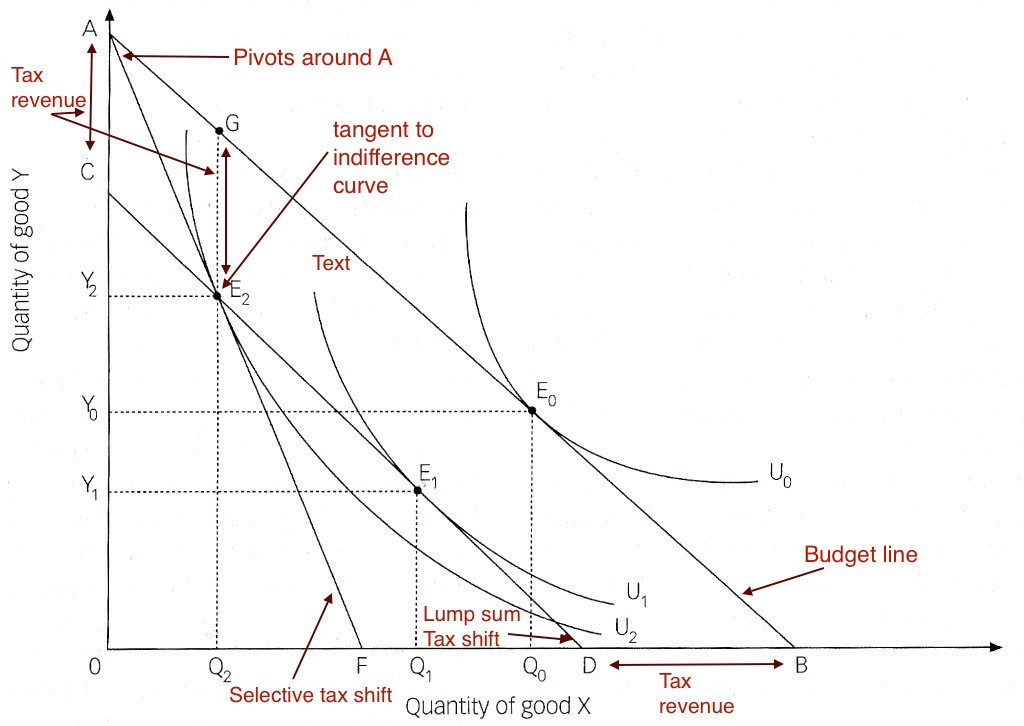
\includegraphics[scale=0.4]{./imgs/111.jpg}
\ra Equilibrium at ...
\ra Lump sum lower income and shifts demand parallel...
\ra Yields revenue $AC$ in terms $Y$ ...
\ra Equilibrium at $E_1$ lower utility but still Pareto efficient.
\ra A lump sum causes normal burden and not excess burden
\ra General taxes resemble lump sum taxes and have no excess burden. They change the relative price of both goods equal and cause a  parallel shift.

\sh{selective tax}
\ra Because Y is not taxed there is no effect but X is tax and so the budget line swivel around $A$ to $AF$
\ra To get the same tax revenue a budget line is drawn from A to a tangent point on $CD$
\ra Equilibrium is at $E_2$ on indifference curve $U_2$
\ra Consumer welfare is lower and indicates the excess burden of selective taxes.
\ra Pareto optimal condition for consumers $MRS_{xy}=\frac{(1+t)P_x}{P_y}$
\ra Pareto optimal condition for producers $MRT_{xy}=\frac{P_x}{P_y}$
\ra Therefore relative prices have been distorted by tax $MRT_{xy} \ne MRS_{xy}$

\sh{Tax neutrality}
\ra Efficient taxes minimise the excess burden.
\rn{1} Tax neutrality: Traditional narrow sense
\rna The tax should not prevent consumers from maximising utility or producers from maximising profit
\rna Rests on the assumption that resources in the economy are allocated efficiently and non-neutral taxes result in a non-optimal reallocation.
\rn{2} Tax neutrality: Modern broader sense
\rna Tax efficiency should also take into account market imperfections as optimality is the exception.
\rna Non-neutral taxes may be beneficial (positive non-neutral) or they may be harmful (negative non-neutral) and by steering economy towards or away from optimality.
\rna A selective tax can move the economy towards optimality and is positive non-neutral.
\rna A general tax is neutral, but may perpetuate existing distortions and is therefore negative non-neutral.

\sh{Magnitude of excess burden}
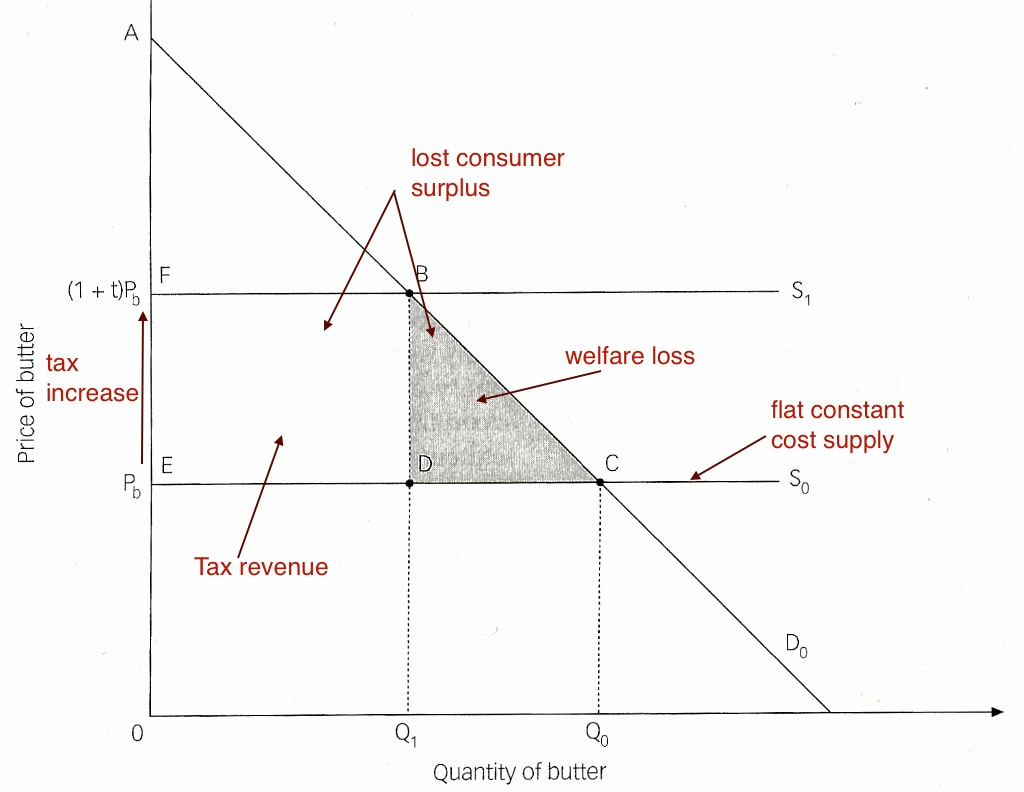
\includegraphics[scale=0.3]{./imgs/112.jpg}
\ra excess burden: $E_b=\frac{1}{2}tP\Delta Q$ \quad$t=BD$ \quad $\Delta Q=DC$ \quad $E_b=BCD$

\sh{Price elasticity}
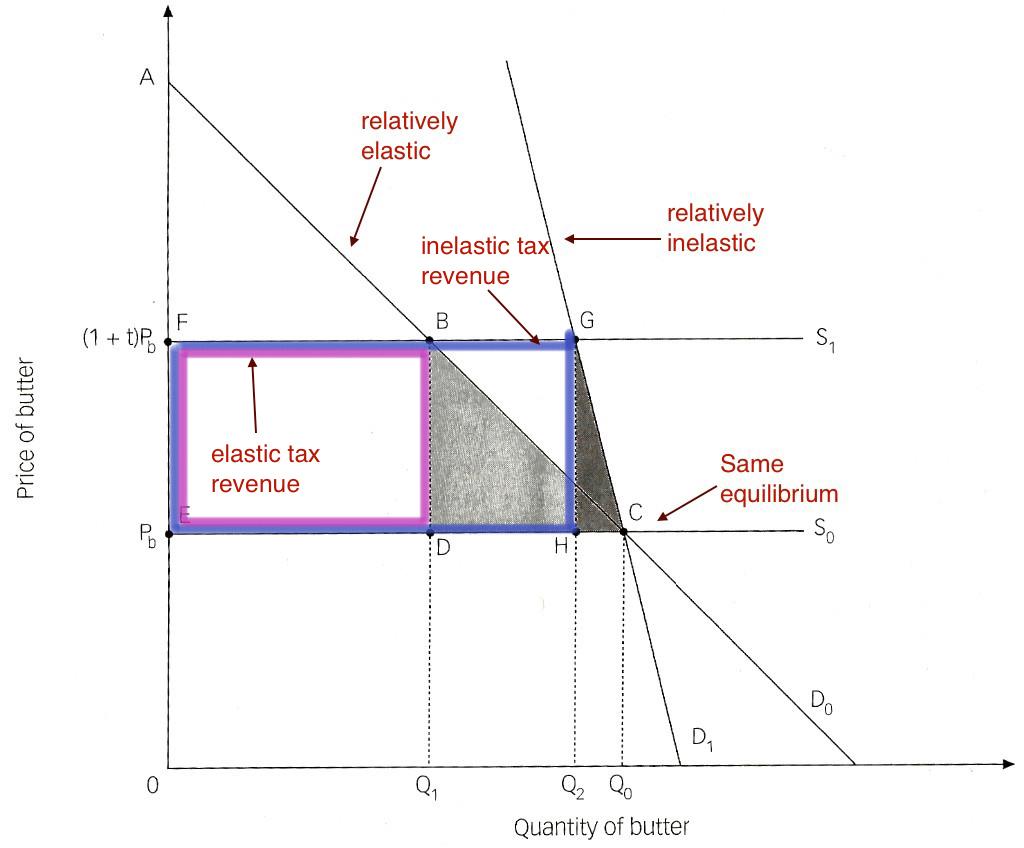
\includegraphics[scale=0.3]{./imgs/113.jpg}
\ra State same equilibrium but small change in quantity for inelastic
\ra The tax revenue on inelastic demand is greater than tax revenue from elastic demand.
\ra Uniform tax rate are not necessarily efficient since higher elasticities of demand should have lower tax rates.
\ra Ramsey's inverse elasticity rule: the excess burden is greater the more elastic the demand curve is and tax revenue is less.
\ra Application of Ramsey's rule leads to problems. Necessities tend to have low elasticity and therefore should have higher taxes, while luxury items tends to have high elasticity and should have low taxes, however expenditure on necessities is higher for low income groups and therefore the tax would be regressive and inequitable. and counter to redistributional objectives.
\ra Tax design is a trade off between equity and efficiency.
\ra $E_b=\frac{1}{2}\epsilon t^2 PQ$. A low $\epsilon$ elasticity means small excess burden. $PQ$ amount spent before tax, so the bigger the larger the excess burden. 

\sh{The tax rate}
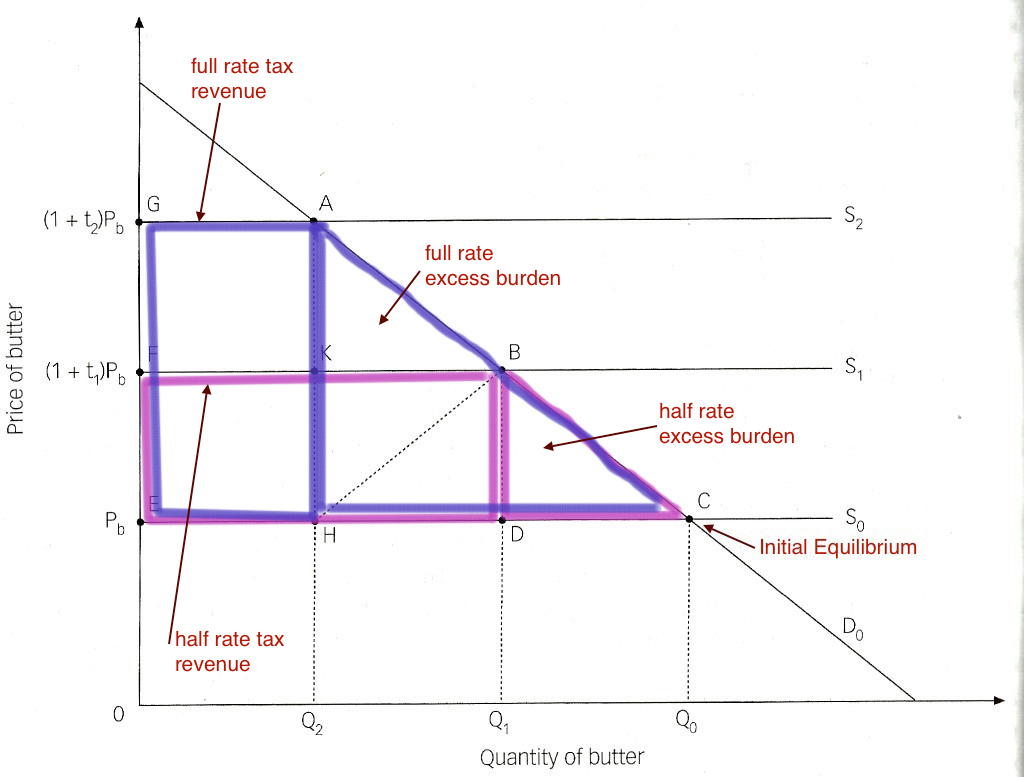
\includegraphics[scale=0.35]{./imgs/114.jpg}
\ra From equilibrium to full tax rate to half tax rate.
\ra Even though tax rate is halved the revenue did not half but the excess burden fell about three quarters.
\ra Efficiency-loss ratio = $\frac{excess\ burden}{tax\ revenue}$ 
\ra As the tax rate increases the excess burden increases as a multiple of the tax rate.
\ra Increases by a multiple of the tax rate (broad-based general taxes are more efficient than narrow-based selective taxes.
\ra low rates of tax on a large number of commodities will produce smaller excess burden and more tax revenue than high tax rate on a few commodities that yield the same total revenue.
\ra Overall economic efficiency can be improved by reducing taxes on goods and services with high efficiency-loss ratios and increasing taxes on goods and services with low efficiency-loss ratios.

\sh{Administrative efficiency}
\ra Compliance costs are tax payers costs incurred in order to meet their tax obligations, such as time spent filling out forms, accountant and lawyers. Significantly greater than government administrative costs.
\ra Administrative efficiency entails minimising both administration cost and compliance costs.
\ra Tax avoidance are the actions taken by tax payers to take advantage of special provisions and tax loopholes in the tax code to reduce their tax liability. Its legal but wasteful as taxpayers make choices on the basis of tax considerations rather than economic considerations which has high opportunity costs. Usually from errors in loosely drafted legislation or bushinesses splitting up to avoid progressive taxes.
\ra Tax evasion is illegal and consists of actions that contravene tax laws. Such as not registering as a tax payer, under-reporting income, more deductions than warranted. Prevalent in the informal sector and a national pastime.
\ra Tax gap is the difference between the tax revenue collected and the expected revenue.
\ra Tax evasion and tax avoidance should be kept to a minimum. 
\ra The golden rule for taxes is simplification. Incentives for tax delinquency should be minimised. High marginal rates should be avoided and the poor should not be taxed. Penalties for tax evasion should be high and actively enforced. 
\ra Taxes should be withheld at source.
\ra Tax morality is the willingness of taxpayers to part with their hard-earned money and is linked to perceptions about the vertical and horizontal equity of taxes and they way in which they are spent.
\ra Taxes should be certain and transparent.

\sh{Flexibility}
\ra Taxes should be flexible enough to provided for changing economic conditions. Taxes can influence economic activity from both supply and demand side. 
\ra Supply side: growth can be influenced by changing the incentive to work and spend. Such as increasing supply of female workers by lower tax on female workers.
\ra Demand side. Smooth out business cycles with stabilisation policy.
\rn{1} Automatic stabiliser. Characterised by built in flexibility, such an a progressive income tax which decreases during times of recession, i.e. relatively more disposable income but lower government revenue. 
\rn{2} Discretionary stabiliser. The timing if discretionary fiscal action is decisive.

%%%%%%%%%%%%%%%%%%%%%%%%%%%%%%%%%%%%%%%
\h{Study Unit 10}

\ra Unit of taxation, whether the taxpayer is single, married, has children. In South Africa its the individual.
\ra Equal marginal sacrifice. income tax rate should increase progressively as taxable income increases.
\ra Marginal tax rates, graduated tax rates on brackets of income and represent the marginal extra tax in respect of extra income.

\sh{Selective tax on labour income}
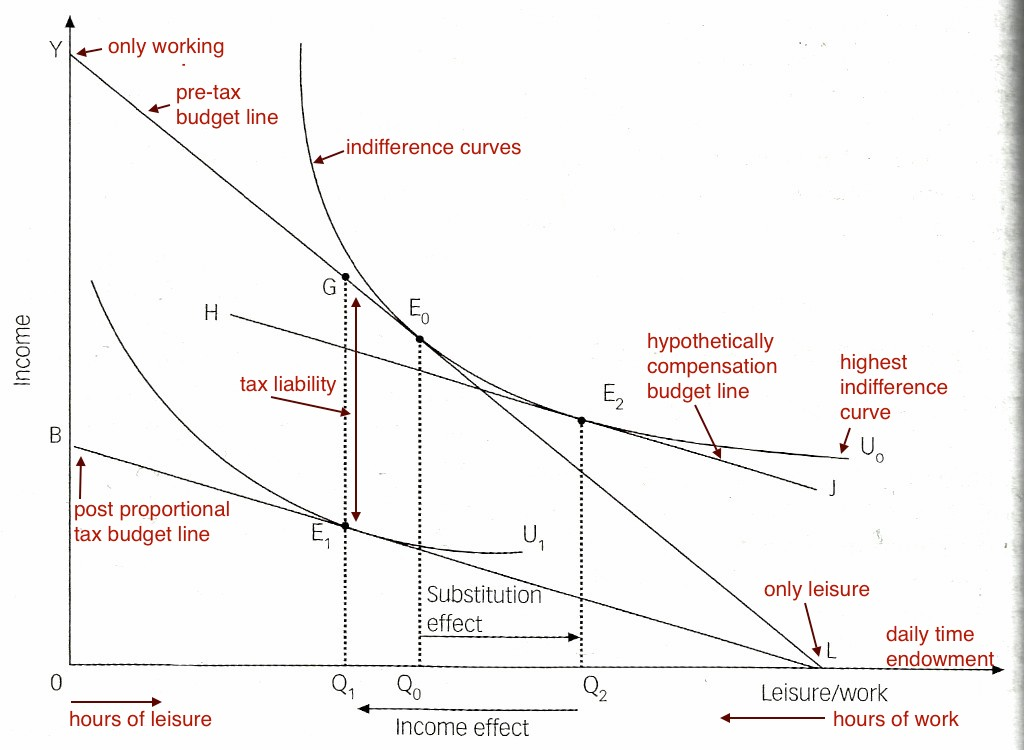
\includegraphics[scale=0.4]{./imgs/121.jpg}
\ra Since leisure cannot be taxed easily a tax on income is in fact a selective tax.
\ra Daily time endowment for either leisure or work. 
\ra Plot budget line from full work to full leisure
\ra Two goods leisure and income
\ra Indifference curves of peters tastes.
\ra Highest indifference curve $U_0$ and equilibrium at ...
\ra After a proportional tax lowers income and swivels budget line down to $BL$ with equilibrium ...
\ra Welfare is lower at $U_1$ tax liability is $E_1G$ and labour increased (not always the case)
\ra Income effect: Working harder to offset loss of income from tax
\ra Substitution effect: (price of one hour of leisure is the hourly wage sacrificed by not working). The tax reduces the opportunity cost of leisure and it becomes cheaper and is hence substituted for work and reduce the quantity of labour supplied.
\ra To show substitution effect on figure. Hypothetically compensating individual with an amount to make him as well off as before budget line shifts to $HJ$ equilibrium is now back at indifference curve $U_0$. This show the substitution of cheaper leisure.
\ra If the income and effect dominates after-tax quantity of labour will increase
\ra If substitution effect dominate after-tax quantity of labour will decrease.
\ra Empirical evidence suggests prime-age men are very insensitive (inelastic) to changes in after-tax income. While married women are quite sensitive to changes in after tax income and labour quantity will be lower after tax.
\ra The size of the income affect is determined by the average tax rate (the amount of tax paid) while the size of substitution effect is determined by the marginal tax rate (additional income sacrificed to tax for additional work effort). As the marginal tax rate becomes larger the incentive for substitution is larger.
\ra For a proportional tax rate the marginal rate equals the average rate whereas fore a progressive tax rate marginal tax rate is higher than average tax rate (higher substitution effect)

\sh{Excess burden of a proportional tax on persona income.}
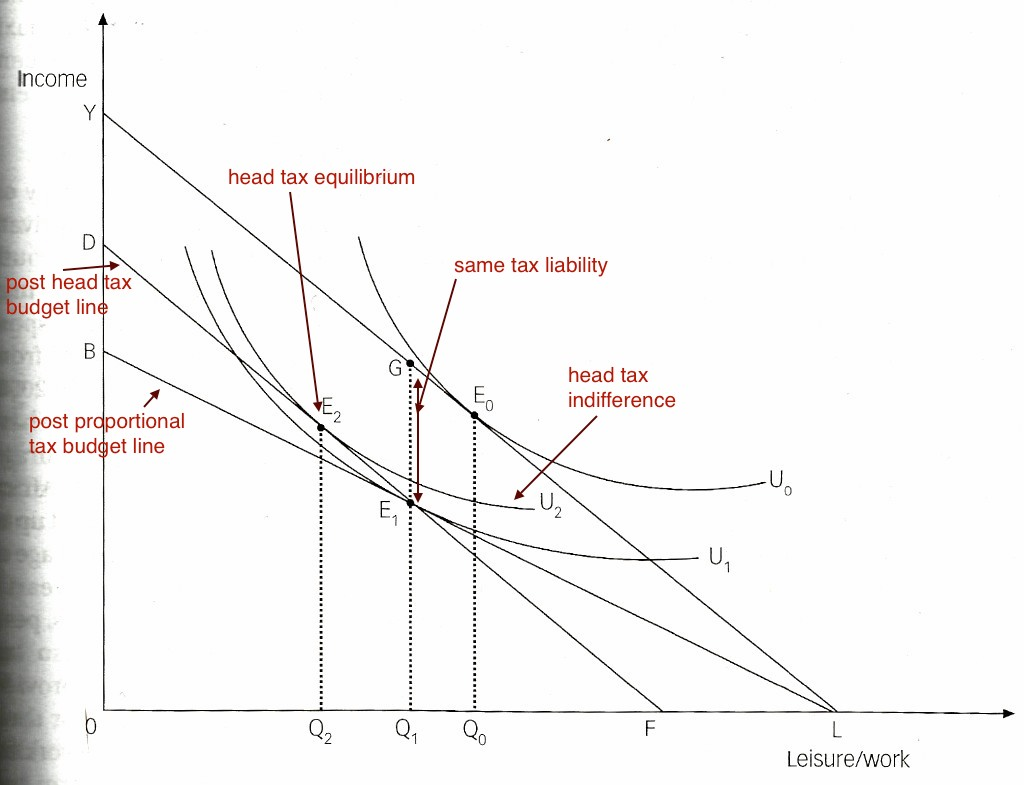
\includegraphics[scale=0.4]{./imgs/122.jpg}
\ra A head tax shifts budget line parallel to $DF$ to intersects at $E_1$ and new equilibrium is at $E_2$ and indifference $U_2$
\ra Works more hours than under proportional tax and has higher welfare.
\ra Difference between proportional and lump sum welfare is excessive burden of proportional tax.
\ra Selective taxes lower the the incentive to work even thought they may lead to increased labour supply. A lump sum tax of equal revenue results in an even larger supply of labour. 
\ra Income taxes are economical inefficient because they distort relative prices, conclusion rest on the inability to tax leisure.
\ra Corlett-Hague rule: tax goods and services complementary to leisure. DVDs, gold clubs, TV. 
\ra Taxing leisure would give an income tax with no excess burden.
\ra Lower marginal tax rates will increase work effort and improve compliance.

\sh{Equity of Income Tax}
\ra If supply of labour is relatively inelastic the burden is on the supplier (employee) (most men)
\ra If the supply curve is less inelastic both employer and employee will share the burden. (married women and mobile high-income professionals
\ra Broadly confirms to the ability to pay principle.

\sh{Administrative efficiency and tax revenue of income tax}
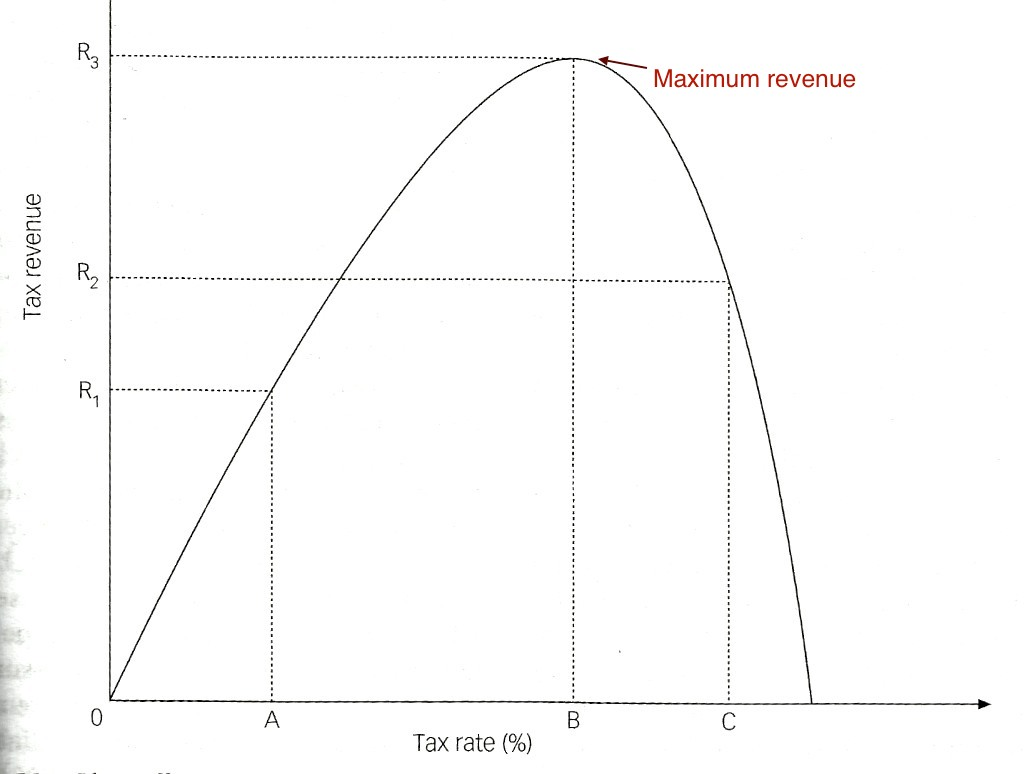
\includegraphics[scale=0.3]{./imgs/124.jpg}
\ra Presumptive taxation involves the use of certain indicators (ownership of certain assets, personal servant, average profit margins) to determine tax liability.
\ra Laffer curve. higher tax rates will not necessarily produce more tax revenue since the tax base will shrink as tax payers reduce their work effort in response to higher rates. 
\ra Tax revenue is the product of the tax rate and the tax base (number of hours worked). At low tax rates an increase in the rate will tend to increase revenues as people will still work more. This will only continue up to a point where revenue will decrease as the substitution effect dominates.
\ra If tax rate is at $C$ authorities should lower the rate. Difficult to determine where on the curve countries are.

\sh{Flexibility of income tax}
\ra Automatic stabiliser rendered useless by inflation.
\ra Bracket creep, process whereby a person is pushed into higher income tax bracket as their nominal income increases, irrespective] of what happens to their real income. Increases tax revenues but is not transparent.
\ra Fiscal drag, damping effect on the economy of the higher tax revenue cruised by bracket creep. Push  government budget into surplus creating a restrictive fiscal policy and can have adverse effect if substantial inflation occurs in recessionary times.
\ra If left unchecked bracket creep undermines vertical equity through inflationary pressures.
\ra Can temper bracket creep by link rates to price index or adjust them on an ad hoc basis. Can also reduce number of tax brackets.

\sh{Capital gains tax}
\ra For
\rn{1} To protect the integrity of personal income tax base, as taxpayers have an incentive to convert income into capital gains to avoid taxation.
\rn{2} To ensure horizontal equity as a capital gain represent an increase in economic power and increases the individuals ability to earn income and to be taxed.
\rn{3} To ensure vertical equity, capital gains accrue mainly to higher income tax payers and are therefore taxed.
\rn{4} To improve economic efficiency
\ra Against
\rn{1} Capital gains taxation is subject numerous  administrative problems, as asset have to be value and the need for up-to-date deeds and registers.
\rn{2} If nominal profits are taxed equity is at risk. Inflation causes imaginary gains and would be unfair to tax.
\rn{3} Capital gains are usually once-off events and tax payers tend to lock in rather than realise investments thereby negatively affect investment. Counter with concessions and lower rates.

%%%%%%%%%%%%%%%%%%%%%%%%%%%%%%%%%%%%%%%
\h{Study Unit 11}
\sh{Unconditional non-matching grants}
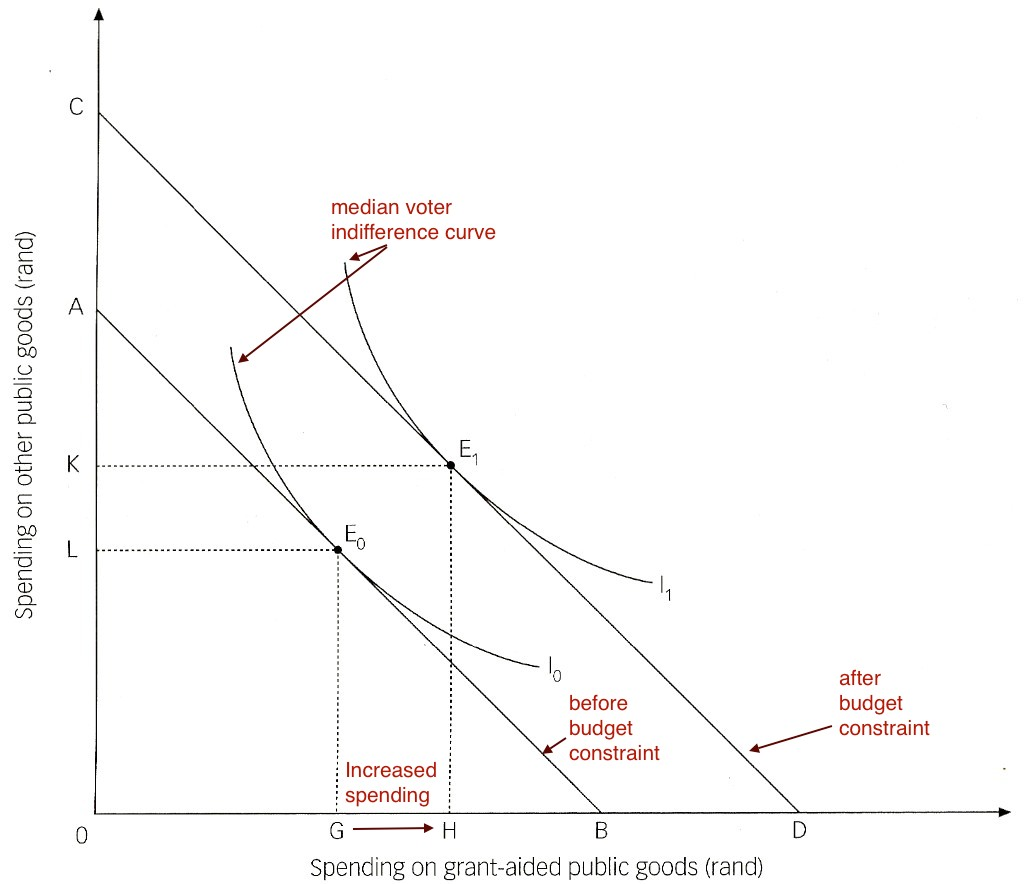
\includegraphics[scale=0.3]{./imgs/171.jpg}
\ra increase income of recipient government but does not alter relative prices.
\ra after grant equilibrium at $E_1$ with higher social welfare
\ra There is an increase in grant-aided public good expenditure but it is less than the size of the grant
\ra Unconditional grant have the least stimulatory effect on grant-aided consumption.

\sh{Conditional non-matching grants}
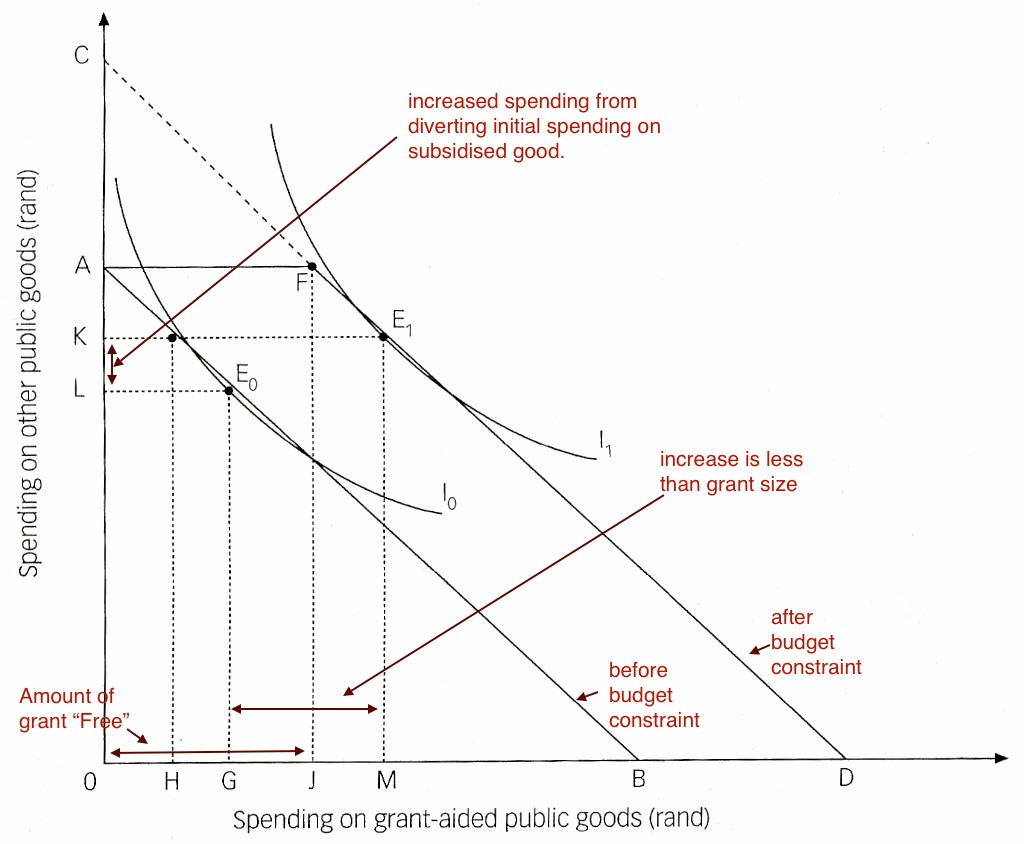
\includegraphics[scale=0.3]{./imgs/172.jpg}
\ra conditional grant shifts budget to $AFD$ by grant size $AF$
\ra $OJ$ is free, 
\ra At $E_1$ extra spending on subsidised good less than grant as part of the initial spending was diverted to other goods $LK$
\ra Best suited it activities consider low priority sub-national government but high priority by national.

\sh{Conditional matching grants (open-ended)}
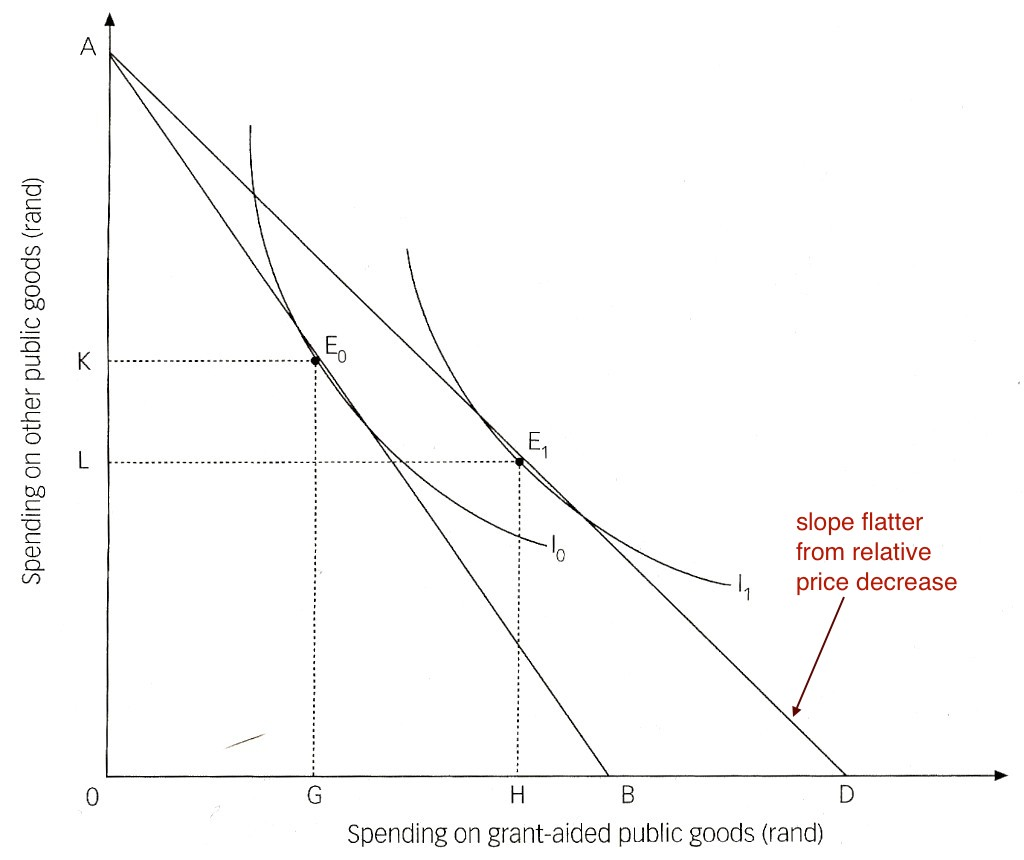
\includegraphics[scale=0.3]{./imgs/173.jpg}
\ra opened-ended can use as much of the grant as long as its matched by local government.
\ra make grant-aided good relativity cheaper
\rn{1} Income Effect public is better off can can consume more of both grant-aided and other public goods.
\rn{2} Substitution effect, substitution of grant-aided goods for other public goods.
\ra net effect of substitution and income effect determines new equilibrium.
\ra If $E_1$ lies to right then both income and substitution effects
\ra If $E_1$ lies to left then income effect dominates substitution effects and less of the grant aided goods is purchased than before.
\ra Opened-ended matching grants most appropriate for correcting inefficiency in public goods with positive externalities because of under providing.

\sh{Conditional matching grants (close-ended)}
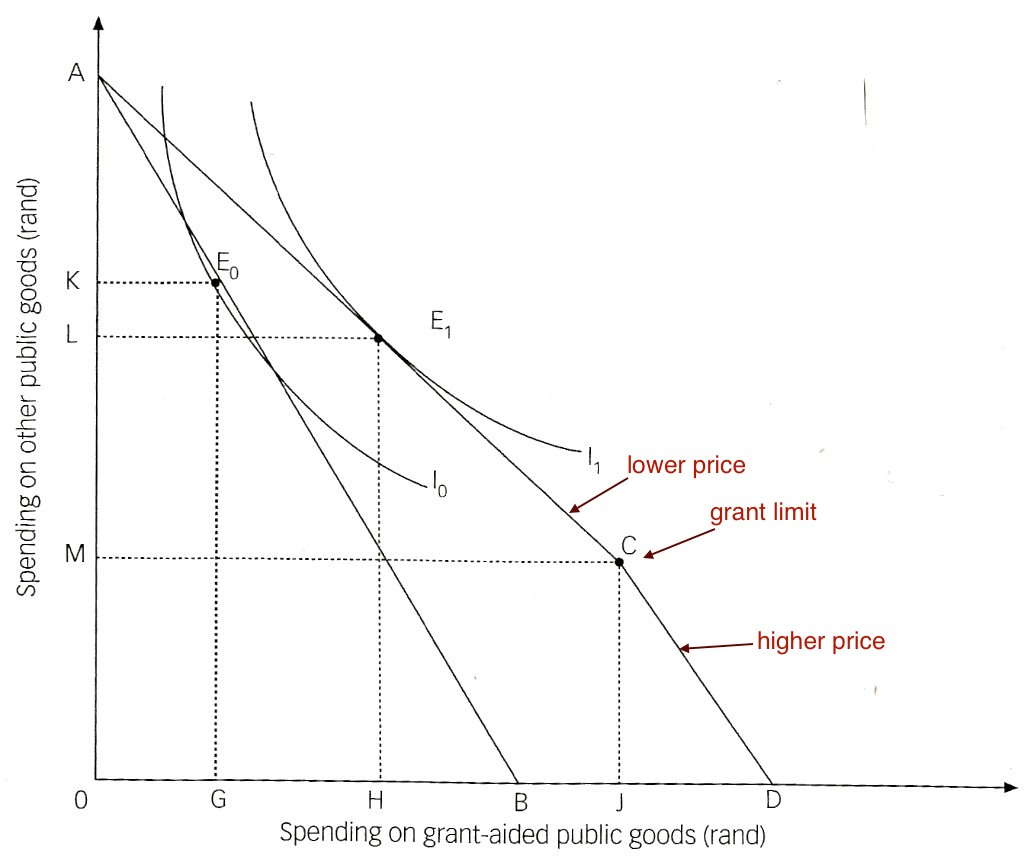
\includegraphics[scale=0.3]{./imgs/174.jpg}
\ra Governments pay some proportion of the cost up to a certain limit.
\ra Governments prefer conditional matching grants closed-ended these allow them to retain control over budgets
-------------------------
\ra conditional non-matching grants to ensure minimum standards
\ra compensation for benefit spill overs conditional matching grants (opened-ended)
\ra conditional matching grant (closed-ended) promoting high priority government activities while retaining budget control.
\ra unconditional non-matching grants for revenue sharing.

-------------------------
\ra \note{incomplete}

\end{document}
